

\documentclass[class = professional, twoside, AutoFakeBold=3.17,AutoFakeSlant=0.2]{gdufe_master_thesis}
% class=academic: 学术学位论文
% class=professional: 专业学位论文
% AutoFakeBold=3.17,AutoFakeSlant=0.2  设置字体伪粗体和伪斜体

% \documentclass[forprint,class=academic]{gdufe_master_thesis}% 选项 forprint: 交付打印时添加, 避免彩色链接字迹打印偏淡.


%% --------biblatex 与cite  bibliographystyle二选一-------------
% 使用biblatex. 如果手写参考文献请注释下两行
\usepackage[style=gb7714-2015, backend=biber]{biblatex}
\addbibresource{reference.bib}

% 不使用biblatex.
% \usepackage{cite} % 使用cite宏包, 以便合并引用文献, 例如 [1-3] 的形式.
% \newcommand{\upcite}[1]{\textsuperscript{\cite{#1}}}  %自定义新命令\upcite, 使参考文献引用以上标出现


%% ----------
% 这两个包是对算法的支持。没写过算法,可以按需修改。
\usepackage{algorithm}
\usepackage{algpseudocode}

% 设置行距
\setlength{\baselineskip}{20pt} \selectfont
\begin{document}
% 中文标题
\title{广东财经大学学术硕士论文 \LaTeX{}模板}

%-----------------------------------------------------------------------------
\pagestyle{empty}
\pdfbookmark[0]{封面}{title}         % 封面页加到 pdf 书签
% 封面文件需要自己在doc文件修改后导出pdf文件,注意修改文件名。
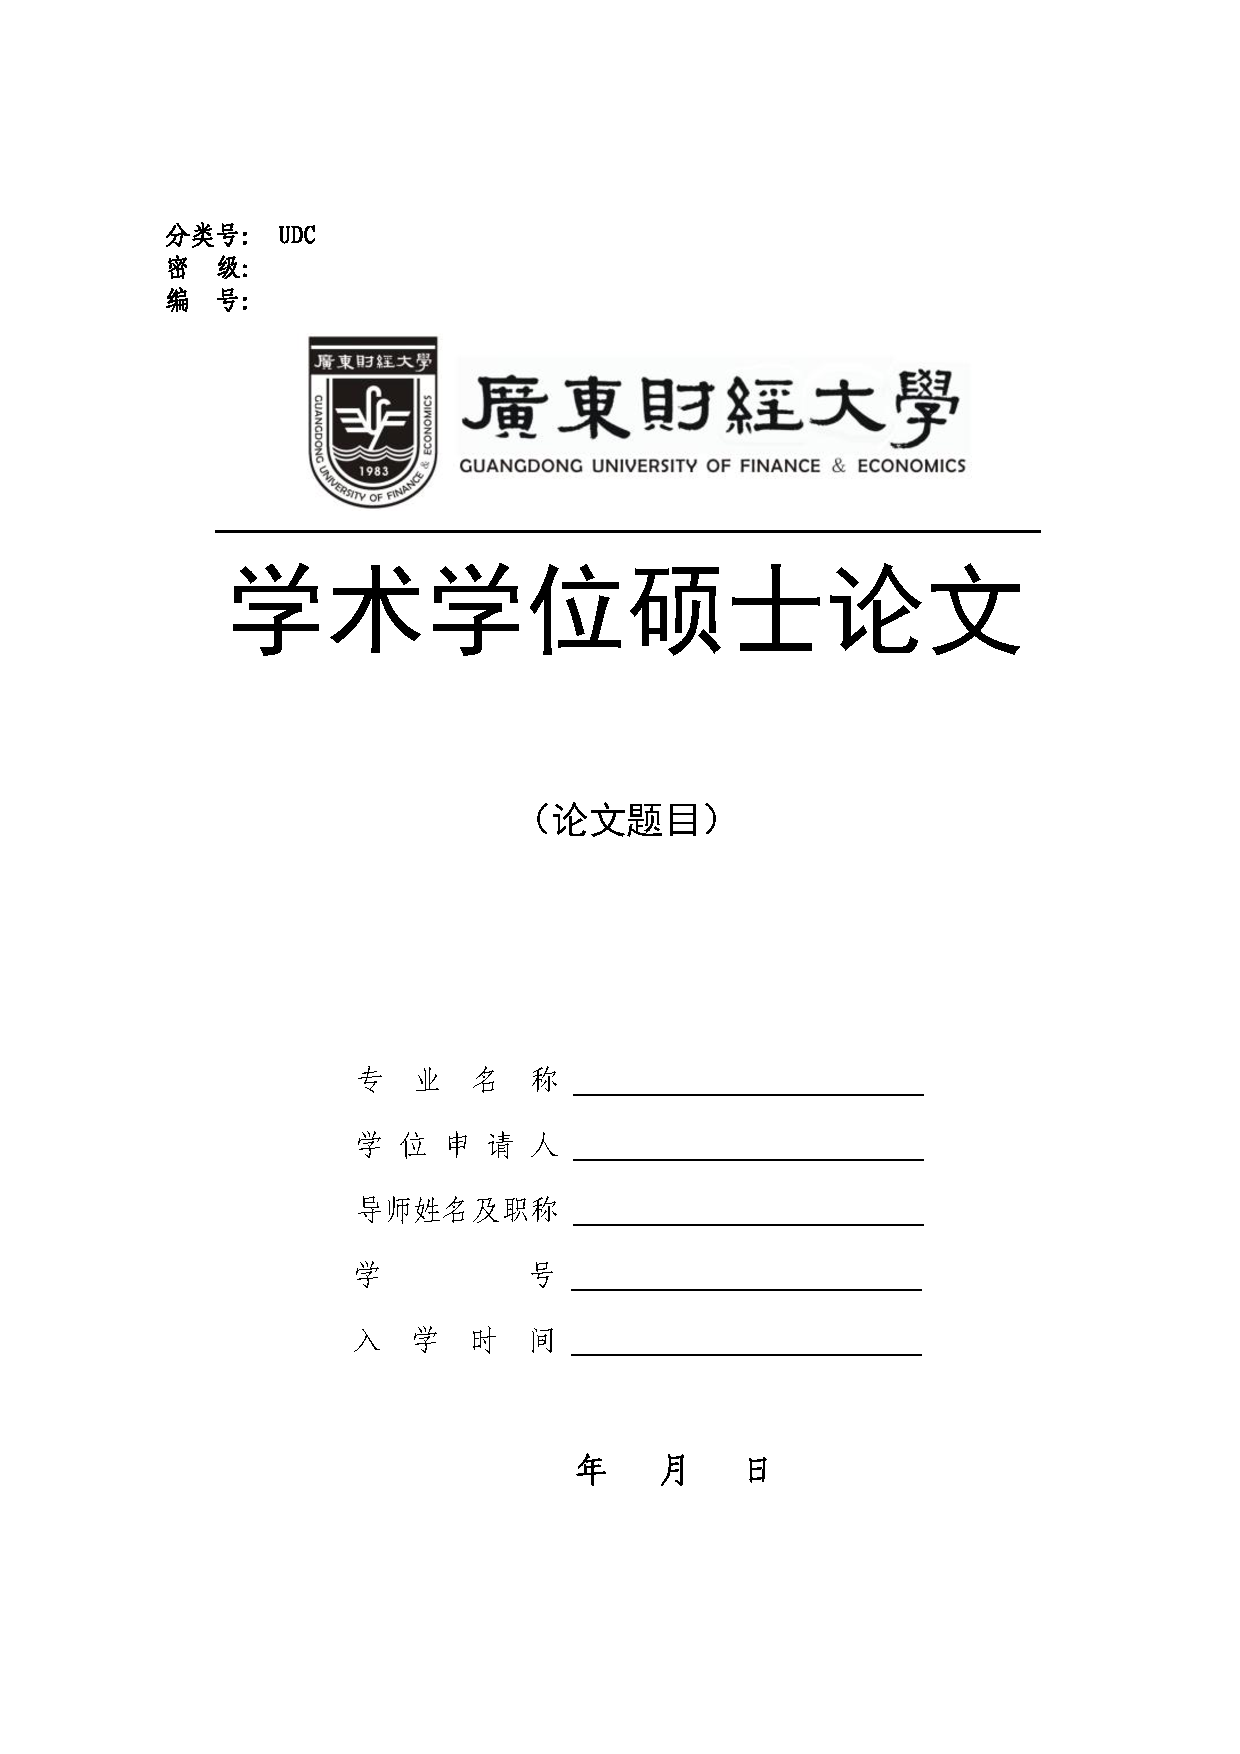
\includepdf[pages=-]{includefile/广东财经大学硕士学位论文封面扉页及声明格式(学术学位).pdf}
% \maketitle
\frontmatter
%-----------------------------------------------------------------------------
% !Mode:: "TeX:UTF-8"

%%% 此部分需要自行填写: (1) 中文摘要及关键词 (2) 英文摘要及关键词
{\setlength{\baselineskip}{20pt} %下文的行距
% \vspace*{0.5cm}
\begingroup
\ctexset{chapter={format+={\centering},
                pagestyle={plain}
        }
        }

\chapter*{\centering \ziju{1} 摘要}
\addcontentsline{toc}{chapter}{摘要}
本文主要介绍和讨论了广东财经大学理工科学年论文的~\LaTeX~模板.
指明了编译方法, 强调了公式排版的一些细节问题, 也指出了一些常见的排版错误.

这是一个示例摘要。本摘要简要介绍了文档的主要内容。文档探讨了相关主题,通过研究与分析,得出了一些有意义的结论。Lorem ipsum dolor sit amet, consectetur adipiscing elit. Sed euismod, velit ac volutpat tincidunt, ipsum nunc fringilla nunc, ac tincidunt risus nunc sed turpis.

这是一个示例摘要。本摘要简要介绍了文档的主要内容。文档探讨了相关主题,通过研究与分析,得出了一些有意义的结论。Lorem ipsum dolor sit amet, consectetur adipiscing elit. Sed euismod, velit ac volutpat tincidunt, ipsum nunc fringilla nunc, ac tincidunt risus nunc sed turpis.
这是一个示例摘要。本摘要简要介绍了文档的主要内容。文档探讨了相关主题,通过研究与分析,得出了一些有意义的结论。Lorem ipsum dolor sit amet, consectetur adipiscing elit. Sed euismod, velit ac volutpat tincidunt, ipsum nunc fringilla nunc, ac tincidunt risus nunc sed turpis.
这是一个示例摘要。本摘要简要介绍了文档的主要内容。文档探讨了相关主题,通过研究与分析,得出了一些有意义的结论。Lorem ipsum dolor sit amet, consectetur adipiscing elit. Sed euismod, velit ac volutpat tincidunt, ipsum nunc fringilla nunc, ac tincidunt risus nunc sed turpis.
这是一个示例摘要。本摘要简要介绍了文档的主要内容。文档探讨了相关主题,通过研究与分析,得出了一些有意义的结论。Lorem ipsum dolor sit amet, consectetur adipiscing elit. Sed euismod, velit ac volutpat tincidunt, ipsum nunc fringilla nunc, ac tincidunt risus nunc sed turpis.

% 这是一个示例摘要。本摘要简要介绍了文档的主要内容。文档探讨了相关主题,通过研究与分析,得出了一些有意义的结论。这是一个示例摘要。本摘要简要介绍了文档的主要内容。文档探讨了相关主题,通过研究与分析,得出了一些有意义的结论。这是一个示例摘要。本摘要简要介绍了文档的主要内容。文档探讨了相关主题,通过研究与分析,得出了一些有意义的结论。这是一个示例摘要。本摘要简要介绍了文档的主要内容。文档探讨了相关主题,通过研究与分析,得出了一些有意义的结论。这是一个示例摘要。本摘要简要介绍了文档的主要内容。文档探讨了相关主题,通过研究与分析,得出了一些有意义的结论。这是一个示例摘要。本摘要简要介绍了文档的主要内容。文档探讨了相关主题,通过研究与分析,得出了一些有意义的结论。这是一个示例摘要。本摘要简要介绍了文档的主要内容。文档探讨了相关主题,通过研究与分析,得出了一些有意义的结论。这是一个示例摘要。本摘要简要介绍了文档的主要内容。文档探讨了相关主题,通过研究与分析,得出了一些有意义的结论。这是一个示例摘要。本摘要简要介绍了文档的主要内容。文档探讨了相关主题,通过研究与分析,得出了一些有意义的结论。这是一个示例摘要。本摘要简要介绍了文档的主要内容。文档探讨了相关主题,通过研究与分析,得出了一些有意义的结论。这是一个示例摘要。本摘要简要介绍了文档的主要内容。文档探讨了相关主题,通过研究与分析,得出了一些有意义的结论。这是一个示例摘要。本摘要简要介绍了文档的主要内容。文档探讨了相关主题,通过研究与分析,得出了一些有意义的结论。这是一个示例摘要。本摘要简要介绍了文档的主要内容。文档探讨了相关主题,通过研究与分析,得出了一些有意义的结论。这是一个示例摘要。本摘要简要介绍了文档的主要内容。文档探讨了相关主题,通过研究与分析,得出了一些有意义的结论。这是一个示例摘要。本摘要简要介绍了文档的主要内容。文档探讨了相关主题,通过研究与分析,得出了一些有意义的结论。


\vskip 1em
%%%%--  关键词 -----------------------------------------%%%%%%%%
%%%%-- 注意: 每个关键词之间用“;”分开,最后一个关键词不打标点符号
\cnkeywords{毕业论文; \LaTeX{}; 模板; 关键词1; 关键词2; 关键词3}


%%====英文摘要==========================%
\chapter*{\bfseries \centering ABSTRACT}
\addcontentsline{toc}{chapter}{ABSTRACT}
\noindent
This thesis is a study on the theory of \dots.

This thesis is a study on the theory of \dots. This thesis is a study on the theory of \dots.

This thesis is a study on the theory of \dots. This thesis is a study on the theory of \dots. This thesis is a study on the theory of \dots. This thesis is a study on the theory of \dots. This thesis is a study on the theory of \dots. This thesis is a study on the theory of \dots. This thesis is a study on the theory of \dots. This thesis is a study on the theory of \dots. This thesis is a study on the theory of \dots. This thesis is a study on the theory of \dots. This thesis is a study on the theory of \dots. This thesis is a study on the theory of \dots.

This thesis is a study on the theory of \dots. This thesis is a study on the theory of \dots. This thesis is a study on the theory of \dots. This thesis is a study on the theory of \dots. This thesis is a study on the theory of \dots. This thesis is a study on the theory of \dots. This thesis is a study on the theory of \dots. This thesis is a study on the theory of \dots. This thesis is a study on the theory of \dots. This thesis is a study on the theory of \dots. This thesis is a study on the theory of \dots. This thesis is a study on the theory of \dots. This thesis is a study on the theory of \dots. This thesis is a study on the theory of \dots. This thesis is a study on the theory of \dots. This thesis is a study on the theory of \dots. This thesis is a study on the theory of \dots. This thesis is a study on the theory of \dots. This thesis is a study on the theory of \dots. This thesis is a study on the theory of \dots. This thesis is a study on the theory of \dots. This thesis is a study on the theory of \dots. This thesis is a study on the theory of \dots. This thesis is a study on the theory of \dots.

\vskip 1em
%%%%%-- Key words --------------------------------------%%%%%%%
%%%%-- 注意: 每个关键词之间用“;”分开,最后一个关键词不打标点符号
\noindent \enkeywords{thesis; \LaTeX{}; template; keyword1; keyword2; keyword3}
\endgroup
}    % 加入摘要.
%==========================把目录加入到书签==============================%%%%%%
\addcontentsline{toc}{chapter}{目录}  % 目录加入到目录
\tableofcontents

\mainmatter
%%%%%%%%%%%%%%%%%%%%%%%%%%--------main matter-------%%%%%%%%%%%%%%%%%%%%%%%%%%%%%%%%%%%%
\setlength{\baselineskip}{20pt} \selectfont
\chapter{撰写、编译、打印\the\baselineskip}
\the\baselineskip
\section{具体使用步骤\the\baselineskip}
\the\baselineskip
\begin{description}

    \item[Step 1]  进入 includefile 文件夹,  打开 abstract.tex, acknowledgment.tex 这两个文档, 分别填写 (1) 中文摘要、英文摘要, (2) 致谢.\the\baselineskip

    \item[Step 2]  打开主文档 gdufe\_master\_thesis\_template.tex, 填写题目、作者等等信息, 撰写正文. 主文档的文件名可以修改,但要求用英文名.

    \item[Step 3]  使用 XeLaTeX 编译. 具体见 \ref{sec-compile} 节.

\end{description}

\section{编译的方法}\label{sec-compile}

默认使用 XeLaTeX 编译, 直接生成~pdf 文件. \the\baselineskip

若另存为新文档, 请确保文档保存类型为 \verb|:UTF-8|. 当然目前很多编辑器默认文字编码为 UTF-8.
WinEdt 9.0 之后的版本都是默认保存为 UTF-8 的. \the\baselineskip

使用~XeLaTeX 编译, 直接生成~pdf 文件.
pdf 文件也可以反向搜索! 双击~pdf 中要修改的文字, 将直接跳转到源文件中相应位置.

如果使用 bib 文件管理参考文献,需要经过
\begin{enumerate}
    \item XeLaTeX

    \item Biber

    \item XeLaTeX

    \item XeLaTeX
\end{enumerate}
四次编译 \the\baselineskip

% \section{文档类型选择}
% 文档类型有 2 种情形:

% \begin{table}[ht]\centering
%     \begin{tabular}{ll}
%         \hline
%         \verb|\documentclass{gdufe\_term\_thesis}|           & 学年论文电子版 \\
%         \verb|\documentclass[forprint]{gdufe\_term\_thesis}| & 毕业论文打印版 \\
%         \hline
%     \end{tabular}
% \end{table}
% 相关解释见下节.

% 2025.5.15更新:只有一个类型 gdufe\_master\_thesis.

\section{打印的问题}
\begin{enumerate}[i)]
    %  \item  论文要求\colorbox{yellow}{单面打印}.
    \item  关于文档选项 forprint: 交付打印时, 建议加上选项 forprint, 以消除链接文字之彩色, 避免打印字迹偏淡.
    \item  打印时留意不要缩小页面或居中. 即页面放缩方式应该是``无''(Adobe Reader XI 是选择``实际大小'').
          有可能页面放缩方式默认为``适合可打印区域'', 会导致打印为原页面大小的 $97\%$.
          文字不要居中打印, 是因为考虑到装订, 左侧的空白留得稍多一点(模板已作预留). \the\baselineskip
    \item  遗留问题: 封面需要打印部重新制作.  校内打印部通常有现成的模板.
          我们自己做的封面, 打印部不一定好用.
\end{enumerate}

\textbf{问}: {\kaishu 生成 PDF 文件时,不能去掉目录和文章的引用彩色方框,请问怎么解决?\the\baselineskip} \the\baselineskip

\textbf{答}: {\kaishu 方框表示超级链接, 只在电脑上看得见. 实际打印时, 是没有的. 另外, 文档类型加选项 forprint 之后, 这些框框会隐掉的. }

\section{文档中的若干命令 \the\baselineskip}
\begin{enumerate}
    \item 若删去参考文献后的\verb|\thispagestyle{plain}|命令则会导致参考文献页显示页眉 \the\baselineskip
\end{enumerate}

\chapter{一些细节的问题}

\section{模板文件结构及功能介绍}

模板文件的结构与功能, 如下表所示:
\begin{table}[ht]\centering
    \begin{tabular}{lll}
        \toprule
        文件夹/文件名                             & 类型     & 功能说明                \\
        \midrule
        gdufe\_master\_thesis\_template.tex & 主文档    & 撰写正文、组织结构           \\
        gdufe\_master\_thesis.cls           & 类文件    & 定义排版格式和命令           \\
        reference.bib                       & bib文件  & 参考文献数据库             \\
        README.md                           & 文本     & 项目说明与使用方法           \\
        includefile/                        & 文件夹    & 存放各章节、摘要、致谢等        \\
        \quad abstract.tex                  & tex文件  & 中英文摘要               \\
        \quad acknowledgment.tex            & tex文件  & 致谢                  \\
        \quad 论文封面、扉页及声明格式.doc              & Word文档 & 编写封面、扉页及声明页         \\
        \quad 论文封面、扉页及声明格式.pdf              & PDF    & 用于编译Tex文件的封面、扉页及声明页 \\
        figures/                            & 文件夹    & 存放图片文件              \\
        \quad gdufelogo.jpg                 & 图片     & 校徽图片                \\
        fonts/                              & 文件夹    & 存放字体文件              \\
        \quad 仿宋\_gb2312.ttf                & 字体     & 仿宋字体                \\
        \bottomrule
    \end{tabular}
    \caption{模板文件结构及功能说明}
\end{table}

无需也不要改变、移动上述文档的位置.

如果不习惯用~\verb|\include{ }|~的方式加入``子文档'', 当然可以把它们合并在主文档, 成为一个文档.
({\kaishu 但是这样并不会给我们带来方便.})

利用~WinEdt~的~Project tree(如图~\ref{fig:1} ), 可以方便地管理这些文件.
\begin{figure}[h]
    \centering
    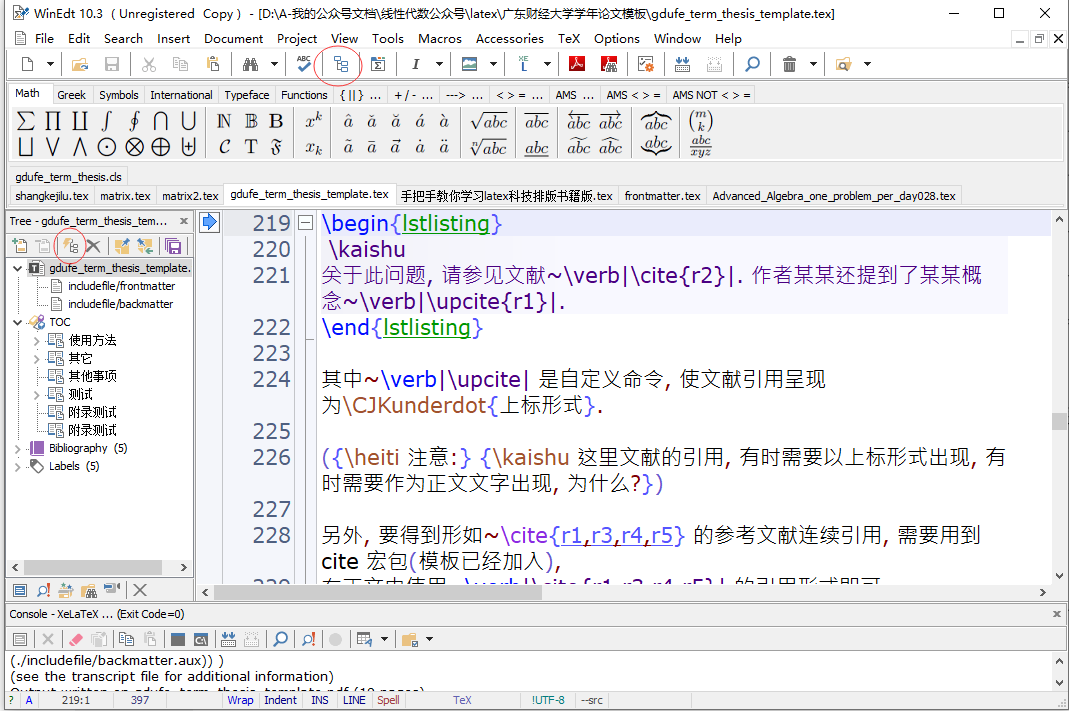
\includegraphics[width=\textwidth]{winedt_file_tree.png}
    \caption{方便在文档内定位的大纲树图}
    \label{fig:1}
\end{figure}

\begin{itemize}
    \item 点击~WinEdt~窗口的~Project Tree~按键;
    \item 再点击~WinEdt~窗口的~Set Main File~按键;
\end{itemize}
接下来的管理, 已经清楚地展示在跳出的窗口中了. 再去处理其他的文件时, 还要点击~WinEdt~窗口的~Remove Main File~按键.

\section{字体调节}

\begin{tabular}{ll}
    \verb|\songti|   & {\songti 宋体}   \\
    \verb|\heiti|    & {\heiti 黑体}    \\
    \verb|\fangsong| & {\fangsong 仿宋} \\
    \verb|\kaishu|   & {\kaishu 楷书}
\end{tabular}


\section{字号调节}
字号命令: \verb|\zihao| \index{zihao}

\begin{tabular}{ll}
    \verb|\zihao{0}|  & \zihao{0}  初号字 English \\
    \verb|\zihao{-0}| & \zihao{-0} 小初号 English \\
    \verb|\zihao{1} | & \zihao{1}  一号字 English \\
    \verb|\zihao{-1}| & \zihao{-1} 小一号 English \\
    \verb|\zihao{2} | & \zihao{2}  二号字 English \\
    \verb|\zihao{-2}| & \zihao{-2} 小二号 English \\
    \verb|\zihao{3} | & \zihao{3}  三号字 English \\
    \verb|\zihao{-3}| & \zihao{-3} 小三号 English \\
    \verb|\zihao{4} | & \zihao{4}  四号字 English \\
    \verb|\zihao{-4}| & \zihao{-4} 小四号 English \\
    \verb|\zihao{5} | & \zihao{5}  五号字 English \\
    \verb|\zihao{-5}| & \zihao{-5} 小五号 English \\
    \verb|\zihao{6} | & \zihao{6}  六号字 English \\
    \verb|\zihao{-6}| & \zihao{-6} 小六号 English \\
    \verb|\zihao{7} | & \zihao{7}  七号字 English \\
    \verb|\zihao{8} | & \zihao{8}  八号字 English \\
\end{tabular}

\section{已加入的常用宏包}
了解类文件cls中已经加载的宏包,在主文档中无须重复加载。
\begin{description}
    \item[amsmath,amssymb]
    \item[cite]  参考文献引用, 得到形如 [3-7] 合并引用文献的样式.
    \item[color,xcolor]  支持彩色.
    \item[enumerate]  方便自由选择 enumerate 环境的编号方式. 比如

          \verb|\begin{enumerate}[(a)]| 得到形如 (a), (b), (c) 的编号.


          \verb|\begin{enumerate}[i)]| 得到形如 i), ii), iii) 的编号.
    \item[tikz] 方便使用tikz作图功能.
    \item[listings] 方便在文档中插入各种程序代码。

\end{description}

另外要说明的是,  itemize, enumerate, description 这三种 list 环境, 已经调节了其间距和缩进,
以符合中文书写的习惯.

\section{标点符号的问题}

建议使用半角的标点符号, 后边再键入一个空格. 特别是在英文书写中要注意此问题!

双引号是由两个左单引号、两个右单引号构成的: \verb|``  ''|. 左单引号在键盘上数字~1 的左边.

但是, 无论您偏向于全角或半角, 强烈建议您使用实心的句号, 只要您书写的是自然科学的文章.
原因可能是因为, 比如使用全角句号的句子结尾处的``$x$。''容易误为数学式~$x_0$(\verb|$x_0$|)吧.



\section{交叉引用的问题}

首先要说明的是,为了得到正确的引用结果,要将tex主文档编译多次。交叉引用是\LaTeX 的强项,它的原理是为被引用对象(图、表、公式、定理等)设置一个标签,例如:~\verb|\label{<标签名>}|, 然后在需要引用的地方用 ~\verb|\ref{<标签名>}|, 就能得到被引用对象的数字编号.
\subsection{参考文献的引用}
 Zotero 软件和期刊网站大多支持导出bib文件, 因此使用 biblatex 和 bib 文件管理参考文献更加方便. 其一可以自动将参考文献表格式按gb7714-2015标准排版. 其二不需要考虑增删移动参考文献位置后重新调整参考文献表. 对此方案不熟悉可以调整回用 {thebibliography} 环境或者自己喜欢的方案.

 {\bfseries 注意:} biblatex 和 cite 包不能同时使用以下两个方案只能选择一个.

\subsubsection{使用 biblatex 管理参考文献}
使用此方案务必取消注释文件开头的\\
\verb|\usepackage[style=gb7714-2015, backend=biber]{biblatex}|\\
\verb|\addbibresource{reference.bib}|\\
以及末尾的\\
\verb|\printbibliography|\\
以及将文件开头的\\
\verb|\usepackage{cite}|\\
\verb|\newcommand{\upcite}|\\
添加注释. 此时可以使用\verb|\cite{}, \parencite{}|引用参考文献

\begin{lstlisting}
详见文献\cite{r1}\parencite{r2}
另见文献\cite[49]{r3}\parencite[106]{r4}
\end{lstlisting}

详见文献\cite{r1}\parencite{r2}
另见文献\cite[49]{r3}\parencite[106]{r4}


使用 \verb|\cite \parencite| 的参考文献是顺序编码制, 其余的引用方式请参考 biblatex, biblatex-gb7714-2015 的文档.\the\baselineskip


\subsubsection{手写 thebibliography 参考文献\the\baselineskip}
\the\baselineskip
不想使用 biblatex 管理参考文献, 要得到形如~{\cite{r1,r3,r4,r5}} 的参考文献连续引用, 需要用到 cite 宏包. 但cite宏包和biblatex宏包有冲突, 因此使用此方案务必注释文件开头的\the\baselineskip\\
\verb|\usepackage[style=gb7714-2015, backend=biber]{biblatex}|\\
\verb|\addbibresource{reference.bib}|\\
以及末尾的\\
\verb|\printbibliography|\\
以及将文件开头的\\
\verb|\usepackage{cite}|\\
\verb|\newcommand{\upcite}|\\
取消注释.

此时的~\verb|\cite{r1,r3,r4,r5}|不是上标引用, 而是正文引用. 想要上标引用可以使用新定义的upcite命令, 如下:
\begin{lstlisting}
    \upcite{r1,r3,r4,r5}
\end{lstlisting}
由于冲突的问题, 请自行查看.


\subsection{定理环境和公式的引用}

本模板定义了7中新定理环境样式, 包括:定理(theorem)、定义(definition)、引理(lemma)、推论(corollary)、例(example)、注(remark). 使用时用如下的格式:
\begin{lstlisting}
\begin{<环境名>}

\end{<环境名>}
\end{lstlisting}

上面的环境名一律是这些英文单词的前四个字母,参见下面的各例:

\begin{theo}[谁发现的]\label{th-abcd}
    最大的正整数是~$1$.
\end{theo}

其源文件如下:

\begin{lstlisting}
 \begin{theo}[谁发现的]\label{th-abcd}
最大的正整数是~$1$.
\end{theo}
\end{lstlisting}

其它环境就不一一举例了。

本模板还提供了证明和解的环境. 证明的环境名为:proof, 解的环境名为solu.

\begin{proof}
    要找到这个最大的正整数, 我们设最大的正整数为~$x$, 则~$x \geqslant 1$, 两边同时乘以~$x$, 得到
    \begin{equation}\label{eq-abc}
        x^2 \geqslant x.
    \end{equation}
    而~$x$ 是最大的正整数, 由~\ref{eq-abc} 式得到
    \[
        x^2 = x.
    \]
    所以
    \begin{equation*}
        x = 1.
    \end{equation*}
\end{proof}

定理~\ref{th-abcd} 是一个重大的发现.

%%%%----- 定义等环境的举例 --------
\begin{defi}[整数]
    正整数(例如 1, 2, 3)、负整数(例如 ${-1}$, $-2$, $-3$)与零(0)合起来统称为{\heiti 整数}.
\end{defi}

\begin{rema}
    整数集合在数学上通常表示为 $\mathbf{Z}$ 或 $\mathbb{Z}$, 该记号源于德语单词 Zahlen(意为``数'')的首字母.
\end{rema}

\begin{prop}
    任意两个整数相加、相减、相乘的结果, 仍然是整数.
\end{prop}

\begin{exam}
    $1+2=3$.
\end{exam}

\begin{coro}
    在整数集合内, 相加、相减、相乘运算是封闭的.
\end{coro}

\section{图形}

支持对~eps, pdf, jpg 等等常见图形格式.

再次\colorbox{red!45}{澄清一个误会}: \LaTeX{} 支持的图形格式绝非 eps 这一种. 无需特意把图片转化为 eps.

用形如~\verb|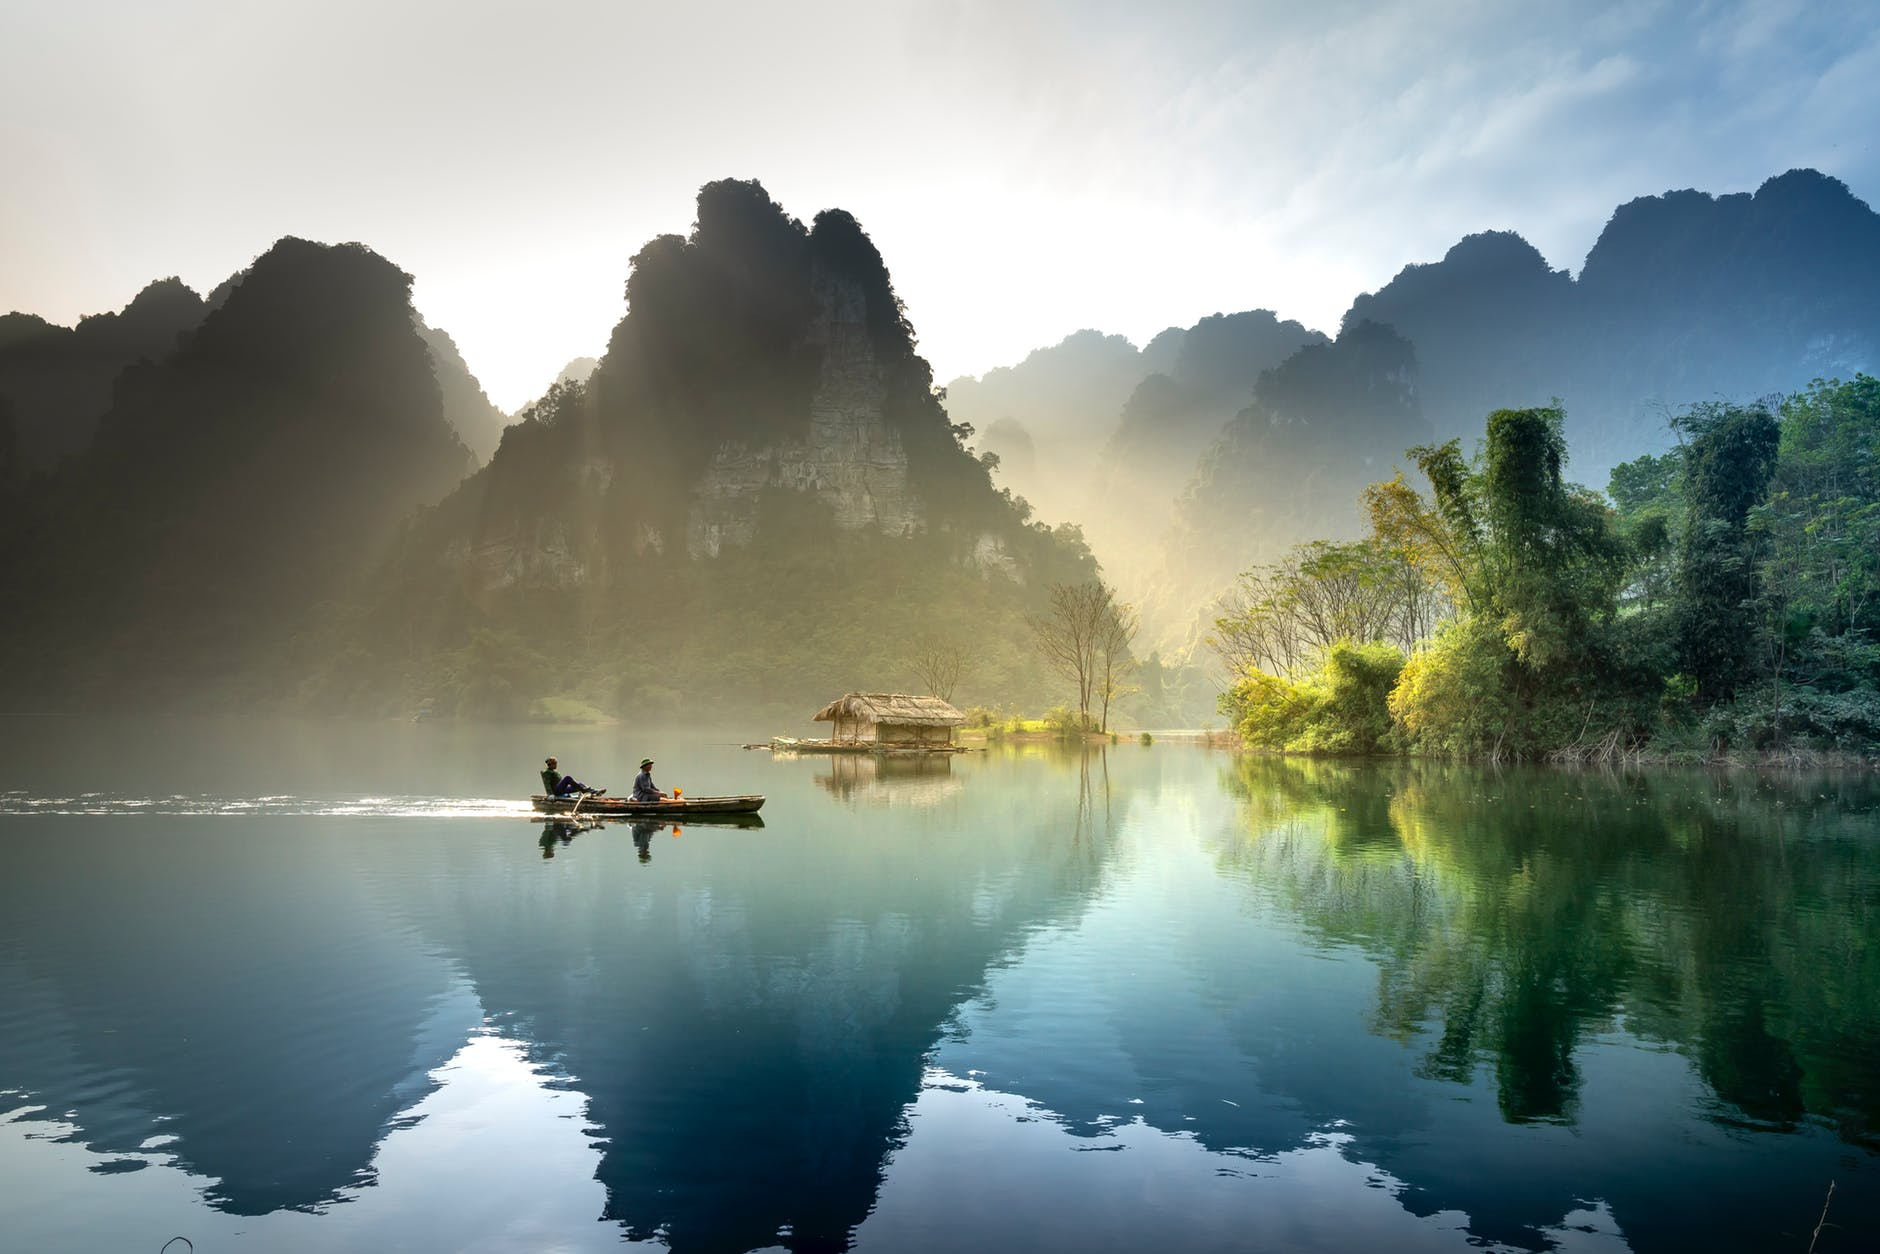
\includegraphics[width=12cm]{lake.jpeg}| 的命令可以纳入图片.

如图~\ref{fig:2} 是一个纳入~jpeg 图片的例子.

\begin{figure}[ht]
    \centering
    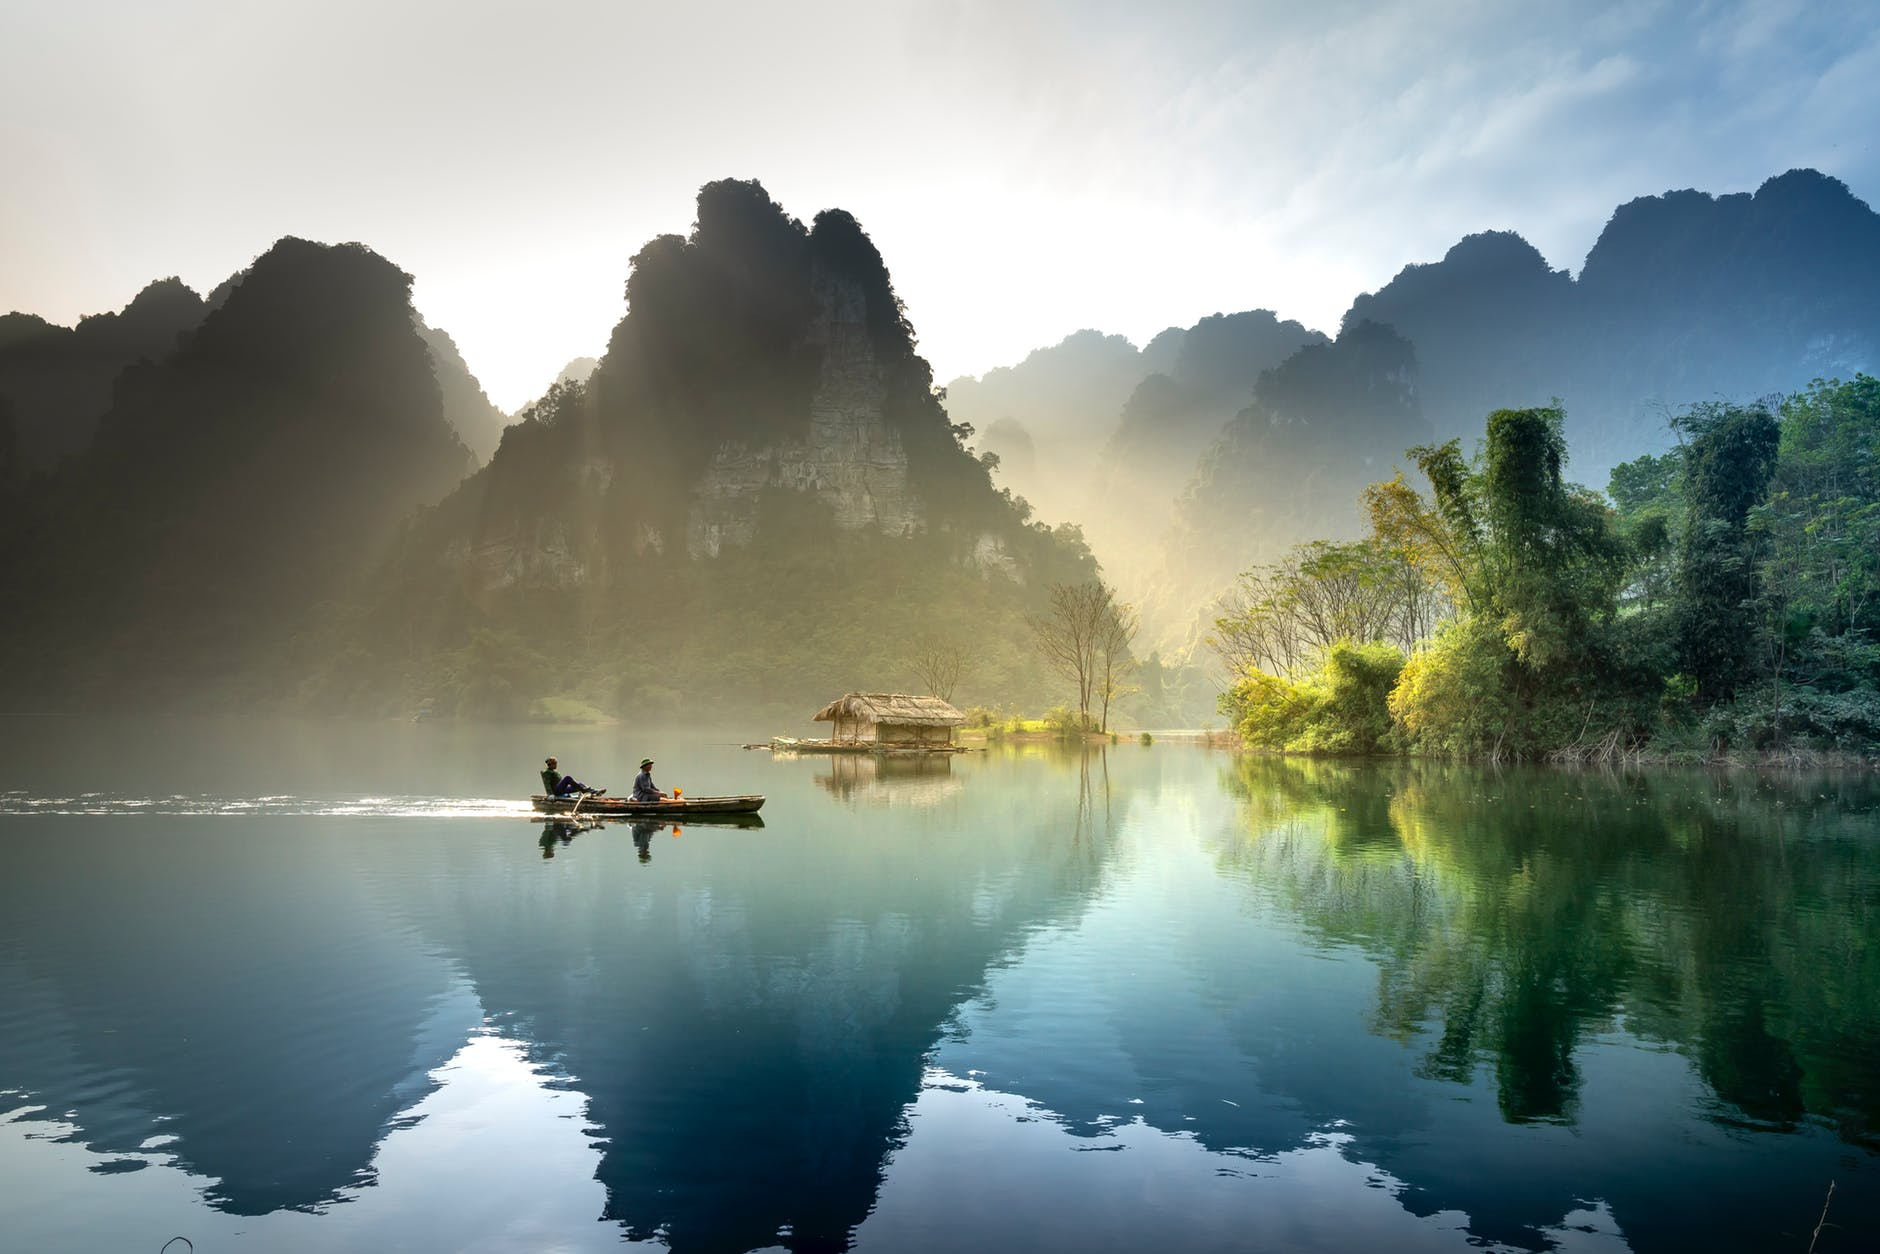
\includegraphics[width=0.5\textwidth]{lake.jpeg}
    \caption{一个彩色 jpeg 图片的例子}
    \label{fig:2}
\end{figure}


\section{表格}
表格问题, 建议使用``三线表'', 如表 \ref{tab:1}.

\begin{table}[ht]
    \centering
    \caption{一般三线表}
    \label{tab:1}
    \begin{tabular}{c c c c c c c c c c c}
        \toprule
        123 & 4   & 5  & 123 & 4 & 5123 & 4 & 5 & 123 & 4 & 5 \\
        \midrule
        67  & 890 & 13 & 123 & 4 & 5123 & 4 & 5 & 123 & 4 & 5 \\
        67  & 890 & 13 & 123 & 4 & 5123 & 4 & 5 & 123 & 4 & 5 \\
        67  & 890 & 13 & 123 & 4 & 5123 & 4 & 5 & 123 & 4 & 5 \\
        \bottomrule
    \end{tabular}
\end{table}


\section{程序代码}

用lstlisting环境可以在文中插入一段代码: \par
\verb|\begin{lstlisting} 代码内容 \end{lstlisting}|. 例如:

\begin{lstlisting}
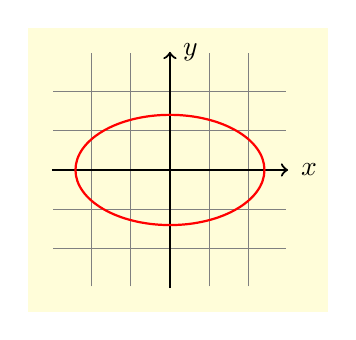
\begin{tikzpicture}[xshift=0.5cm]
   \draw[draw=yellow!15,fill=yellow!15](-1.8,-1.8)rectangle(2,1.8);
   \draw[help lines, step=0.5cm](-1.48,-1.48)grid(1.48,1.48);
   \draw[->,thick] (-1.5,0)--(1.5,0)node[right=1pt]{$x$};
   \draw[->,thick](0,-1.5)--(0,1.5)node[right=1pt]{$y$};
   \draw[color=red,thick](0,0)ellipse[x radius=1.2cm,y radius=0.7cm];
 \end{tikzpicture}
 \end{lstlisting}

输出为:\quad
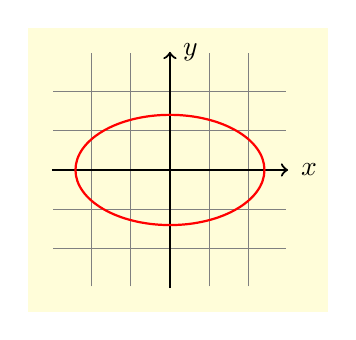
\begin{tikzpicture}[xshift=0.5cm]
    \draw[draw=yellow!15,fill=yellow!15](-1.8,-1.8)rectangle(2,1.8);
    \draw[help lines, step=0.5cm](-1.48,-1.48)grid(1.48,1.48);
    \draw[->,thick] (-1.5,0)--(1.5,0)node[right=1pt]{$x$};
    \draw[->,thick](0,-1.5)--(0,1.5)node[right=1pt]{$y$};
    \draw[color=red,thick](0,0)ellipse[x radius=1.2cm,y radius=0.7cm];
\end{tikzpicture}
%%============================================================================================================%%%

\chapter{显示测试}
\section{字体测试}
中文宋体正常 \textbf{中文宋体加粗} \textit{中文宋体斜体}

English \textbf{English} \textit{English}
\section{数学公式测试}
带编号公式
\begin{equation}
    \int_0^1 x^2 \mathrm{d}x = \frac{1}{3}.
\end{equation}

不带编号公式
\begin{equation*}
    \int_0^1 x^2 \mathrm{d}x = \frac{1}{3}.
\end{equation*}

\section{图片测试}
单图测试
\begin{figure}[h]
    \centering
    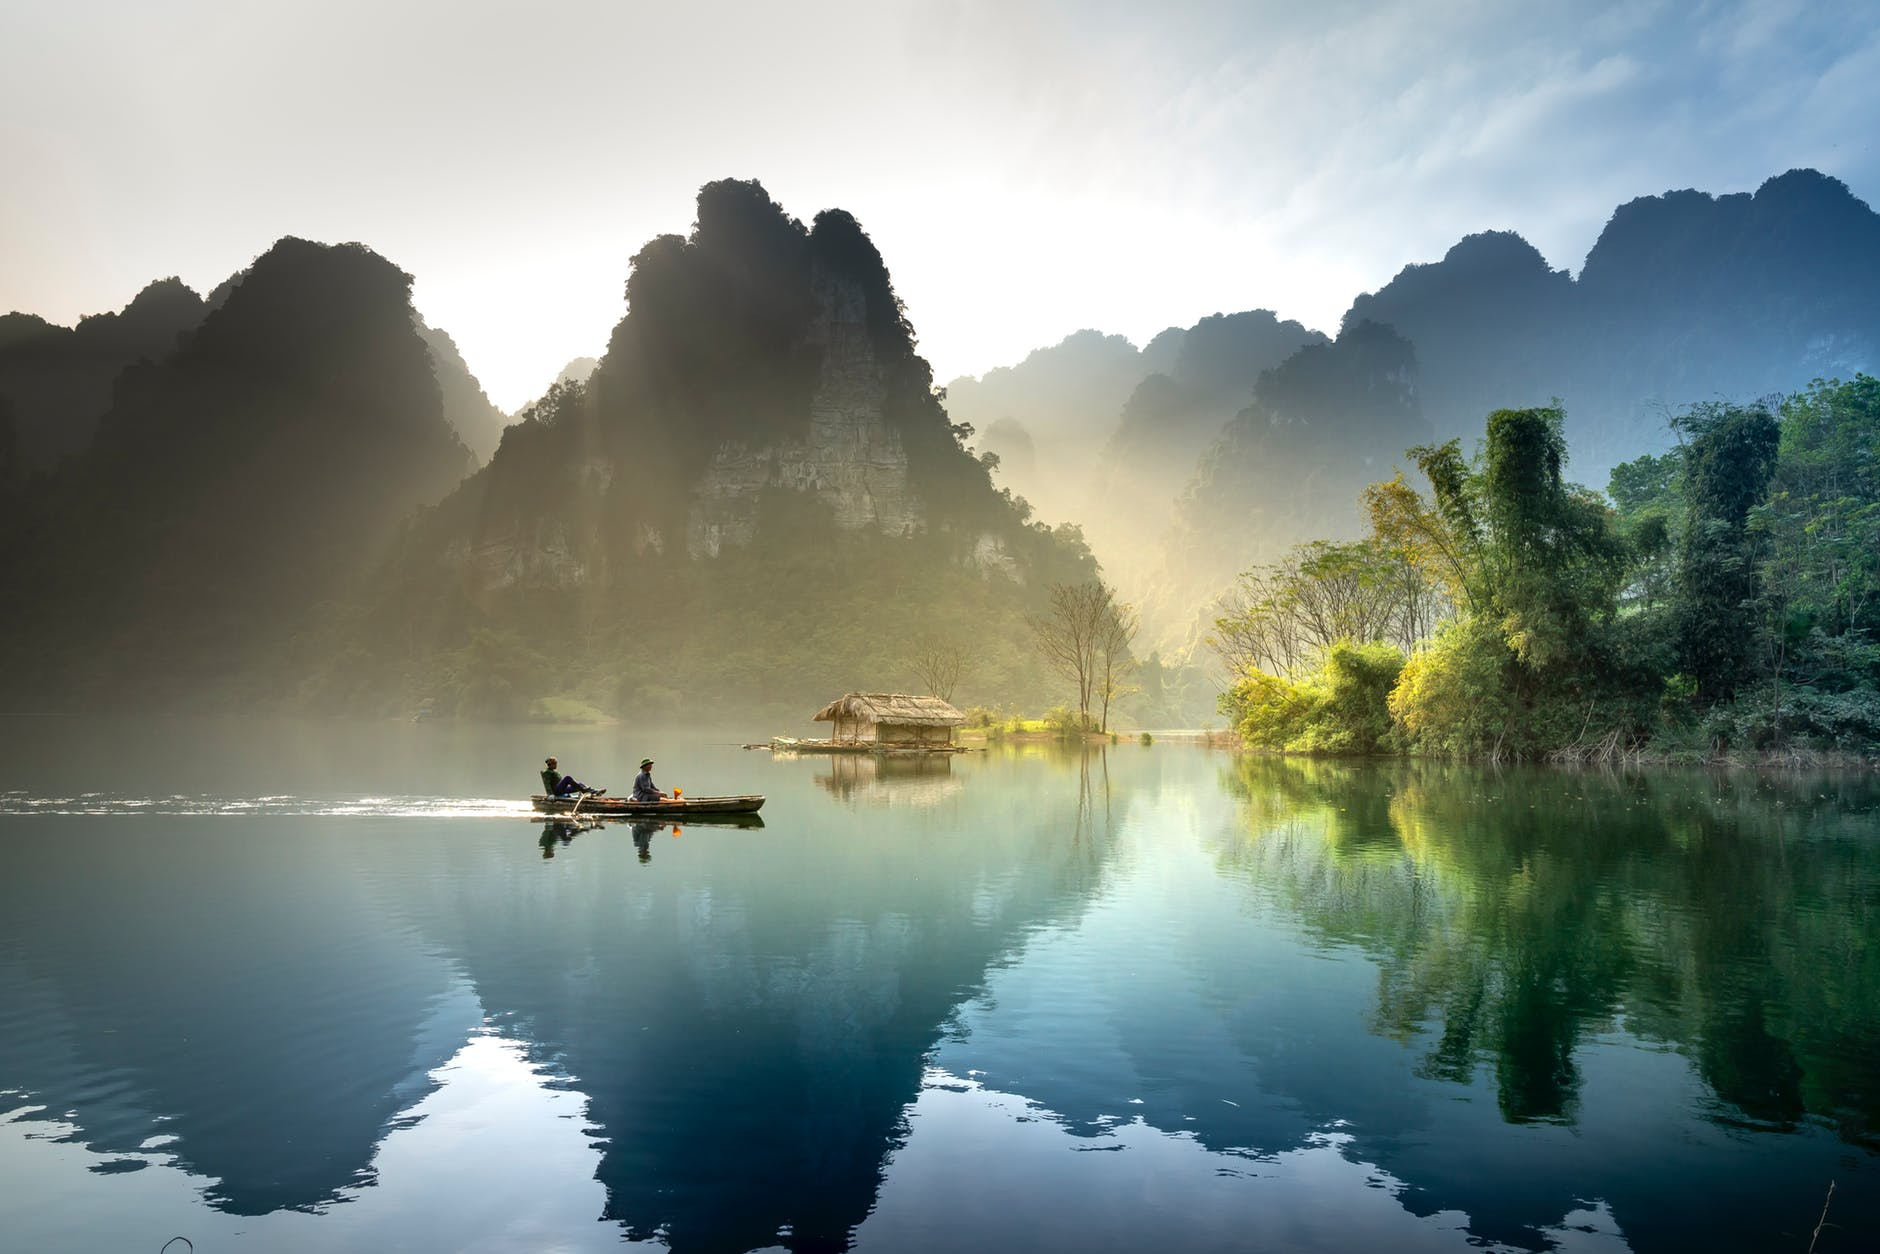
\includegraphics[width=0.8\textwidth]{lake.jpeg}
    \caption{单图片}
    \label{fig:singlePic}
\end{figure}

多图测试1
\begin{figure}[h]
    \centering
    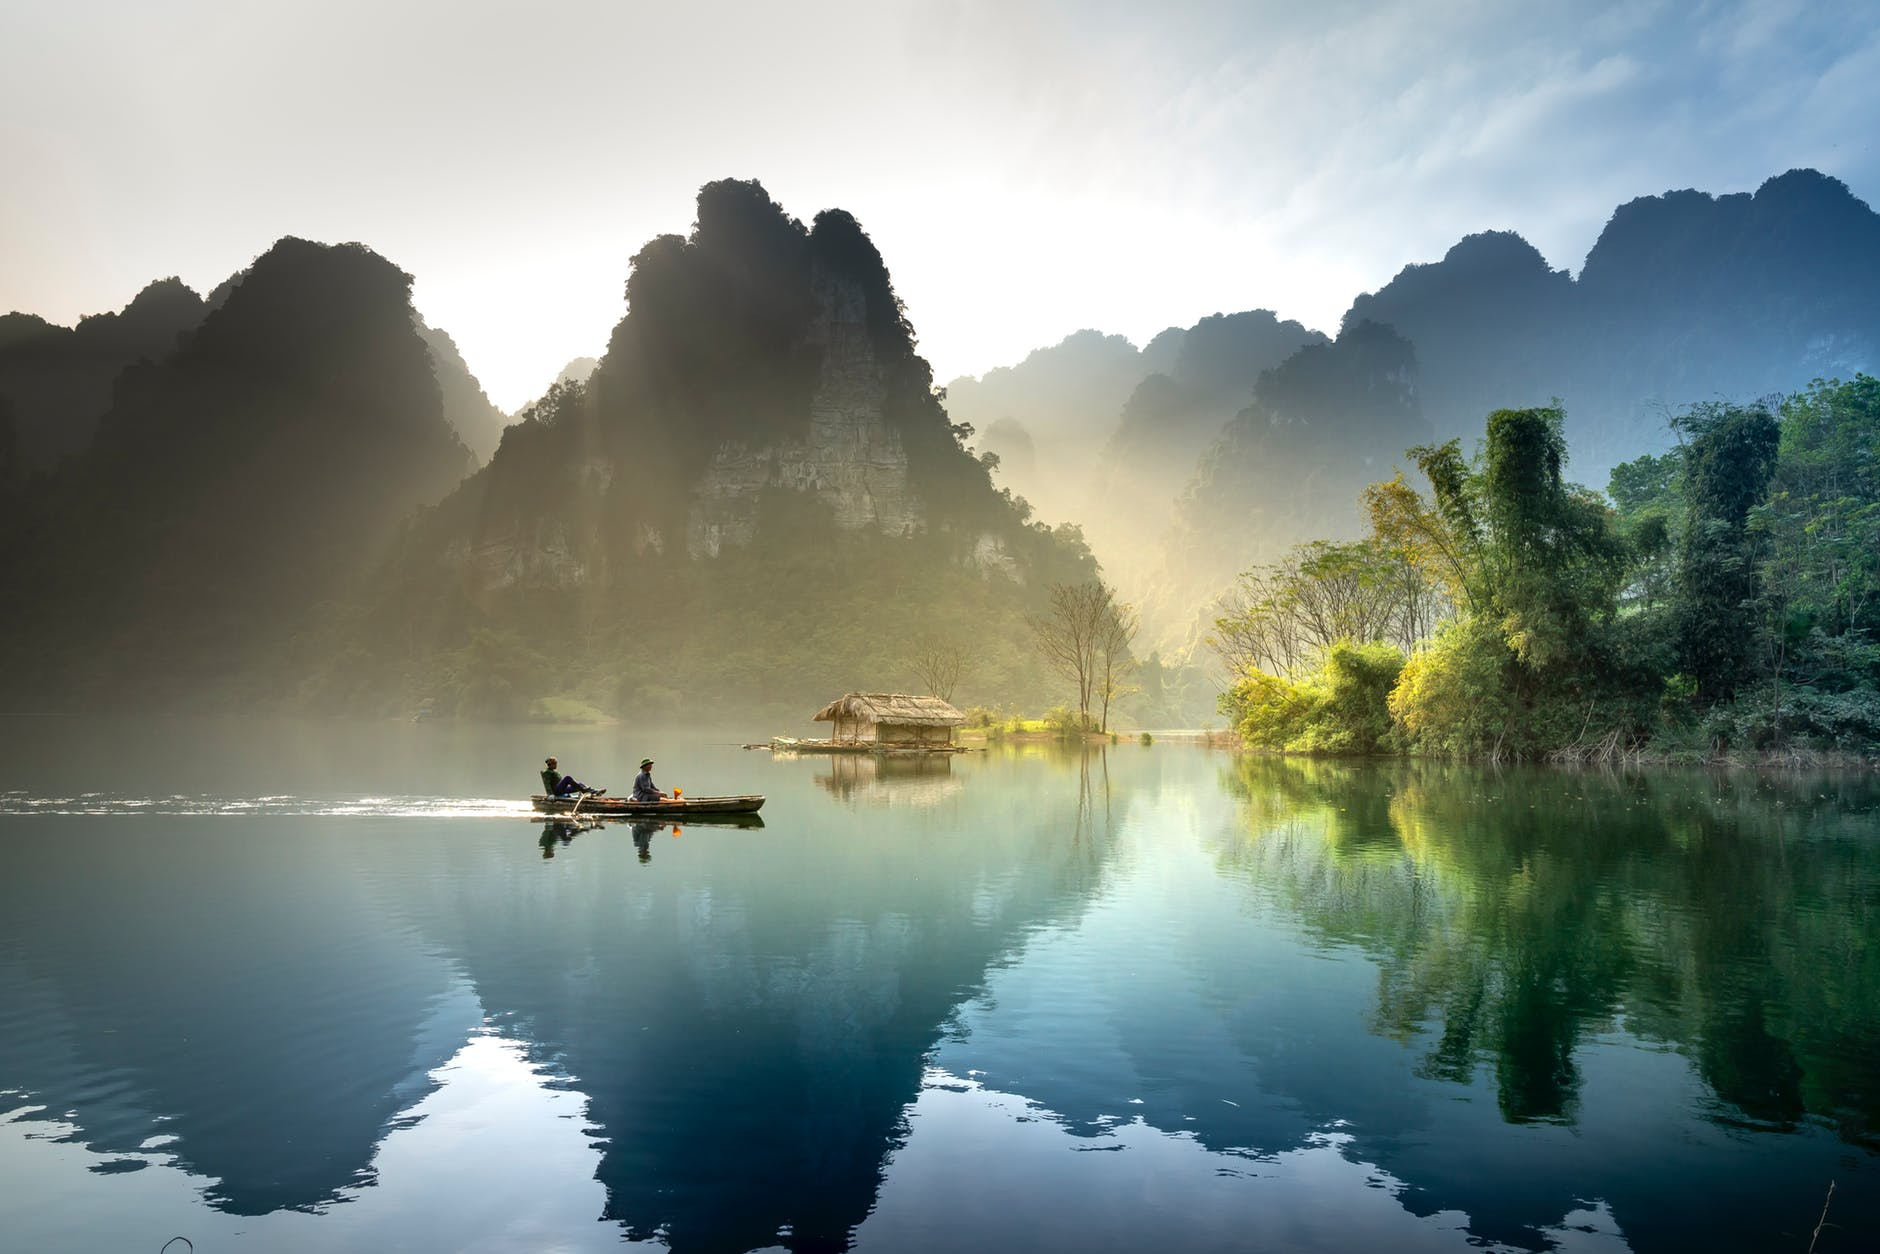
\includegraphics[width=0.3\textwidth]{lake.jpeg}\hfill
    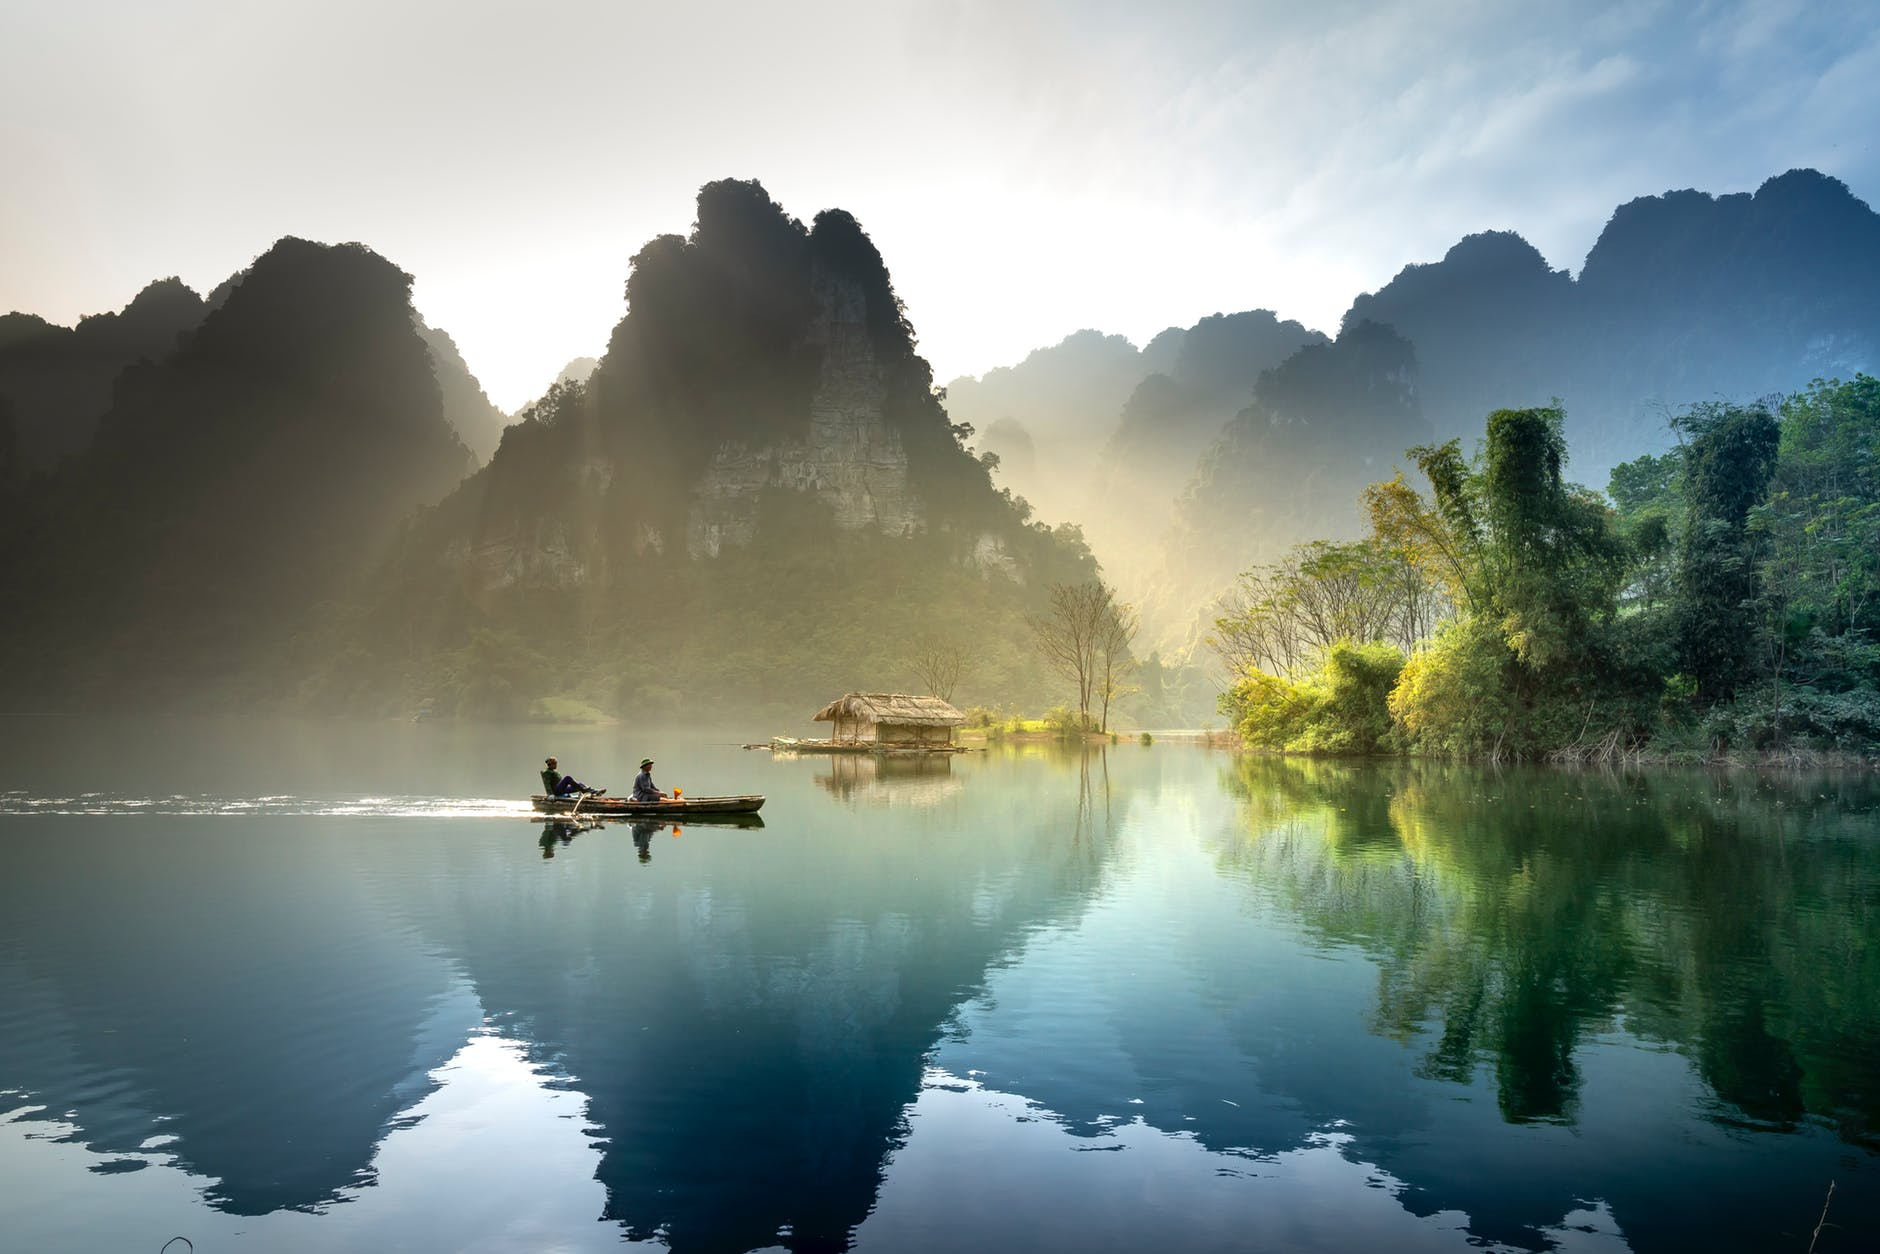
\includegraphics[width=0.3\textwidth]{lake.jpeg}\hfill
    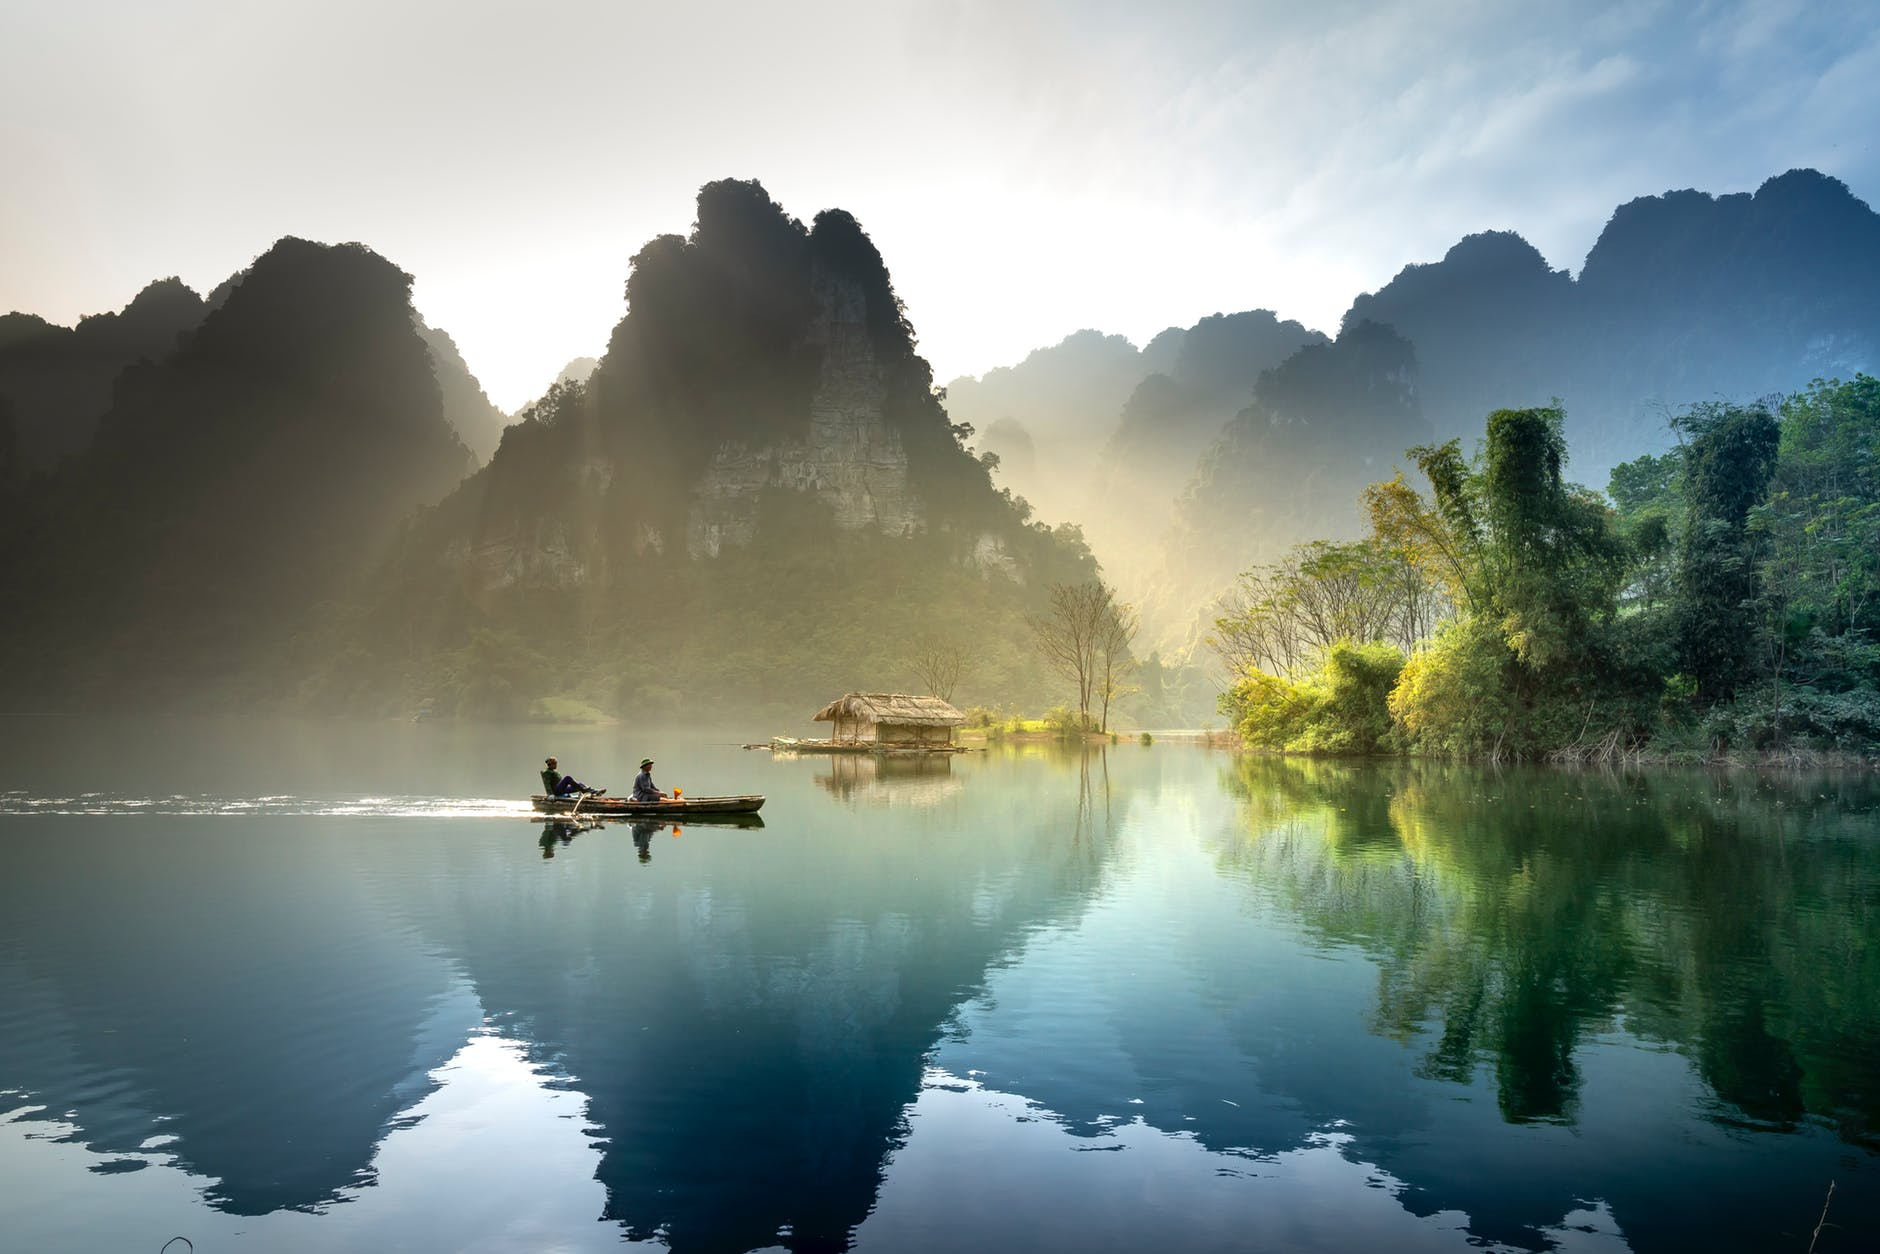
\includegraphics[width=0.3\textwidth]{lake.jpeg}
    \caption{多图片1:珠江三角洲投资管理体制市场化改革(1985---2005)}
    {\zihao{5} \songti 资料来源:xxx}
    \label{fig:MultiPic1}
\end{figure}

多图测试2
\begin{figure}[h]
    \centering
    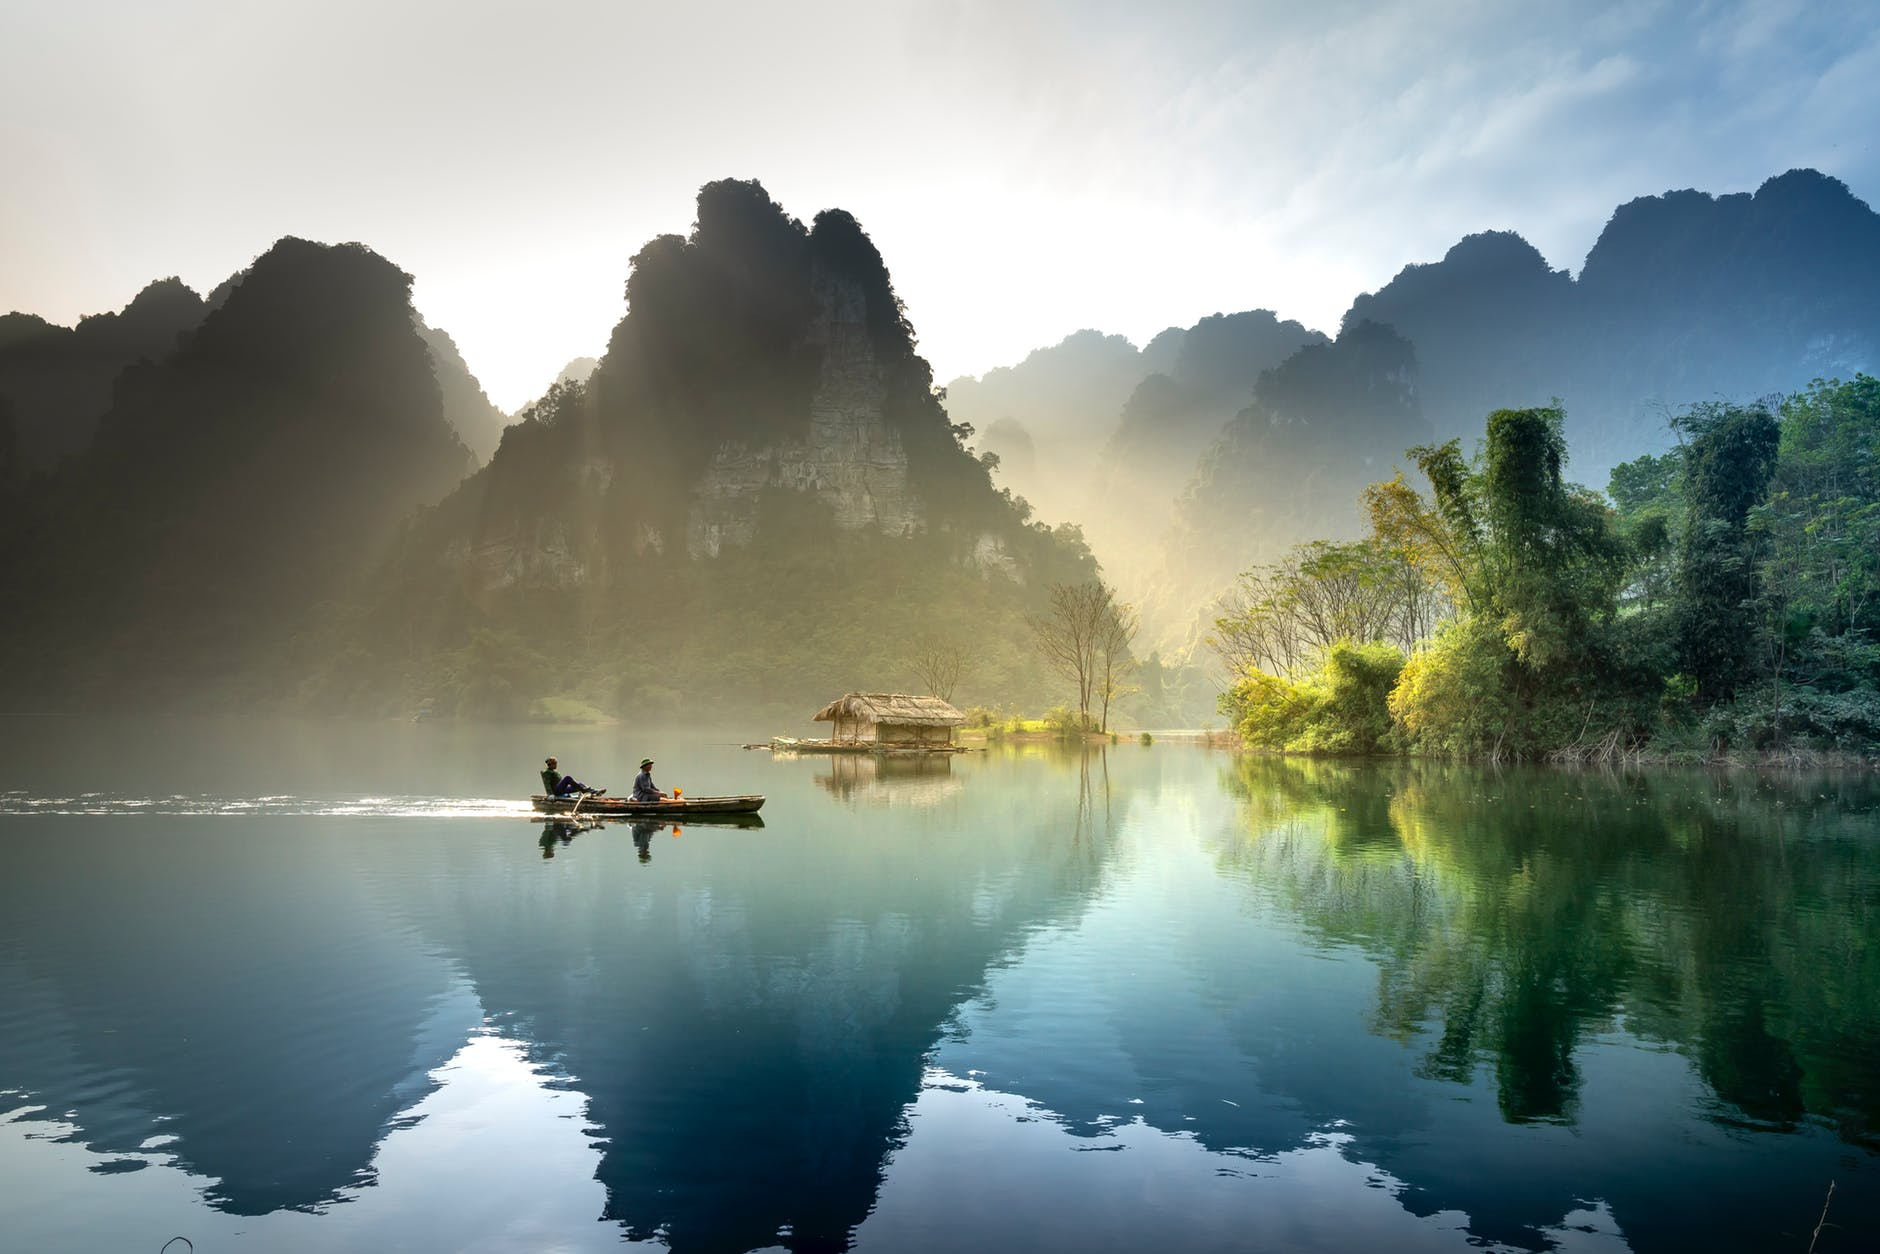
\includegraphics[width=0.5\textwidth]{lake.jpeg}\\
    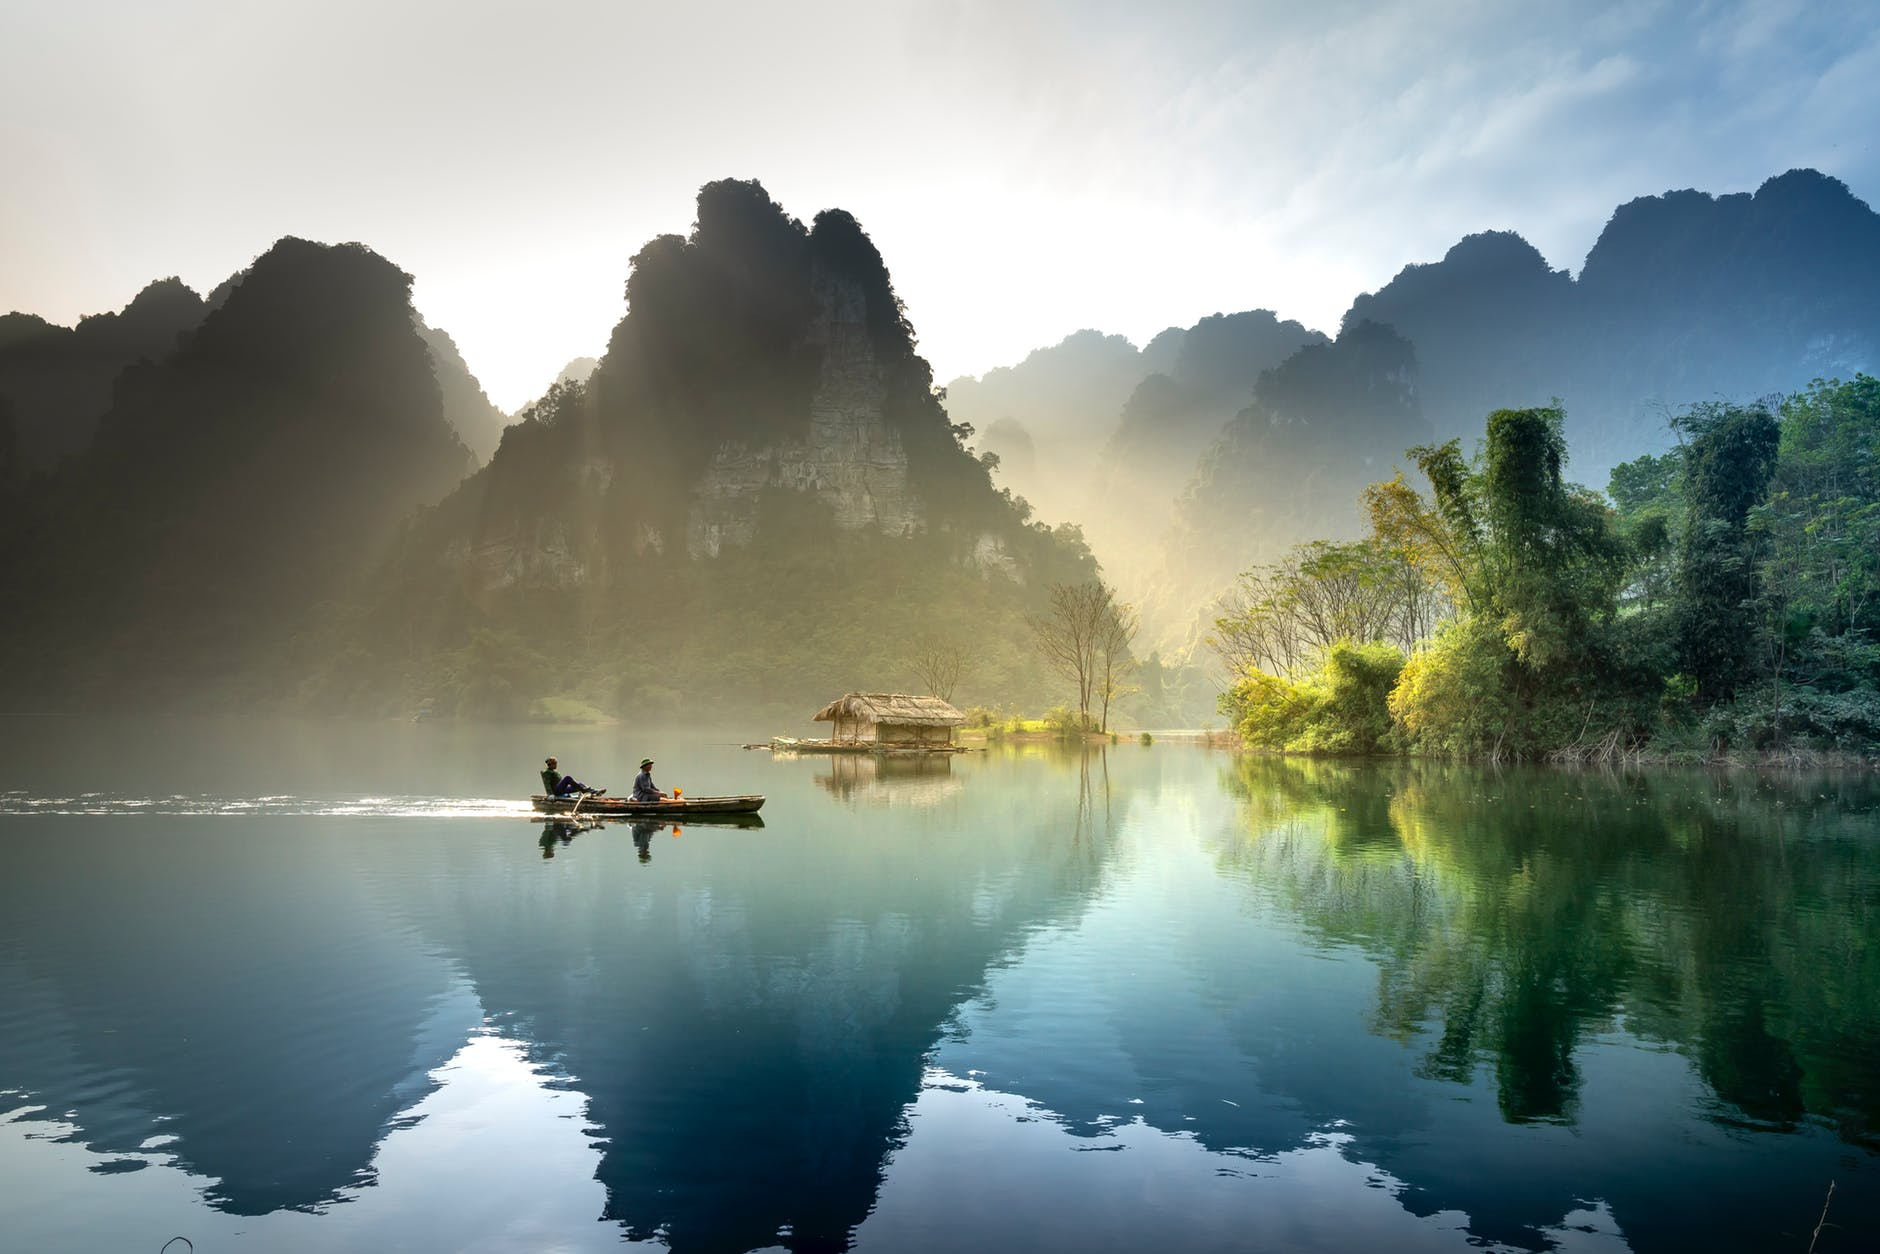
\includegraphics[width=0.5\textwidth]{lake.jpeg}\\
    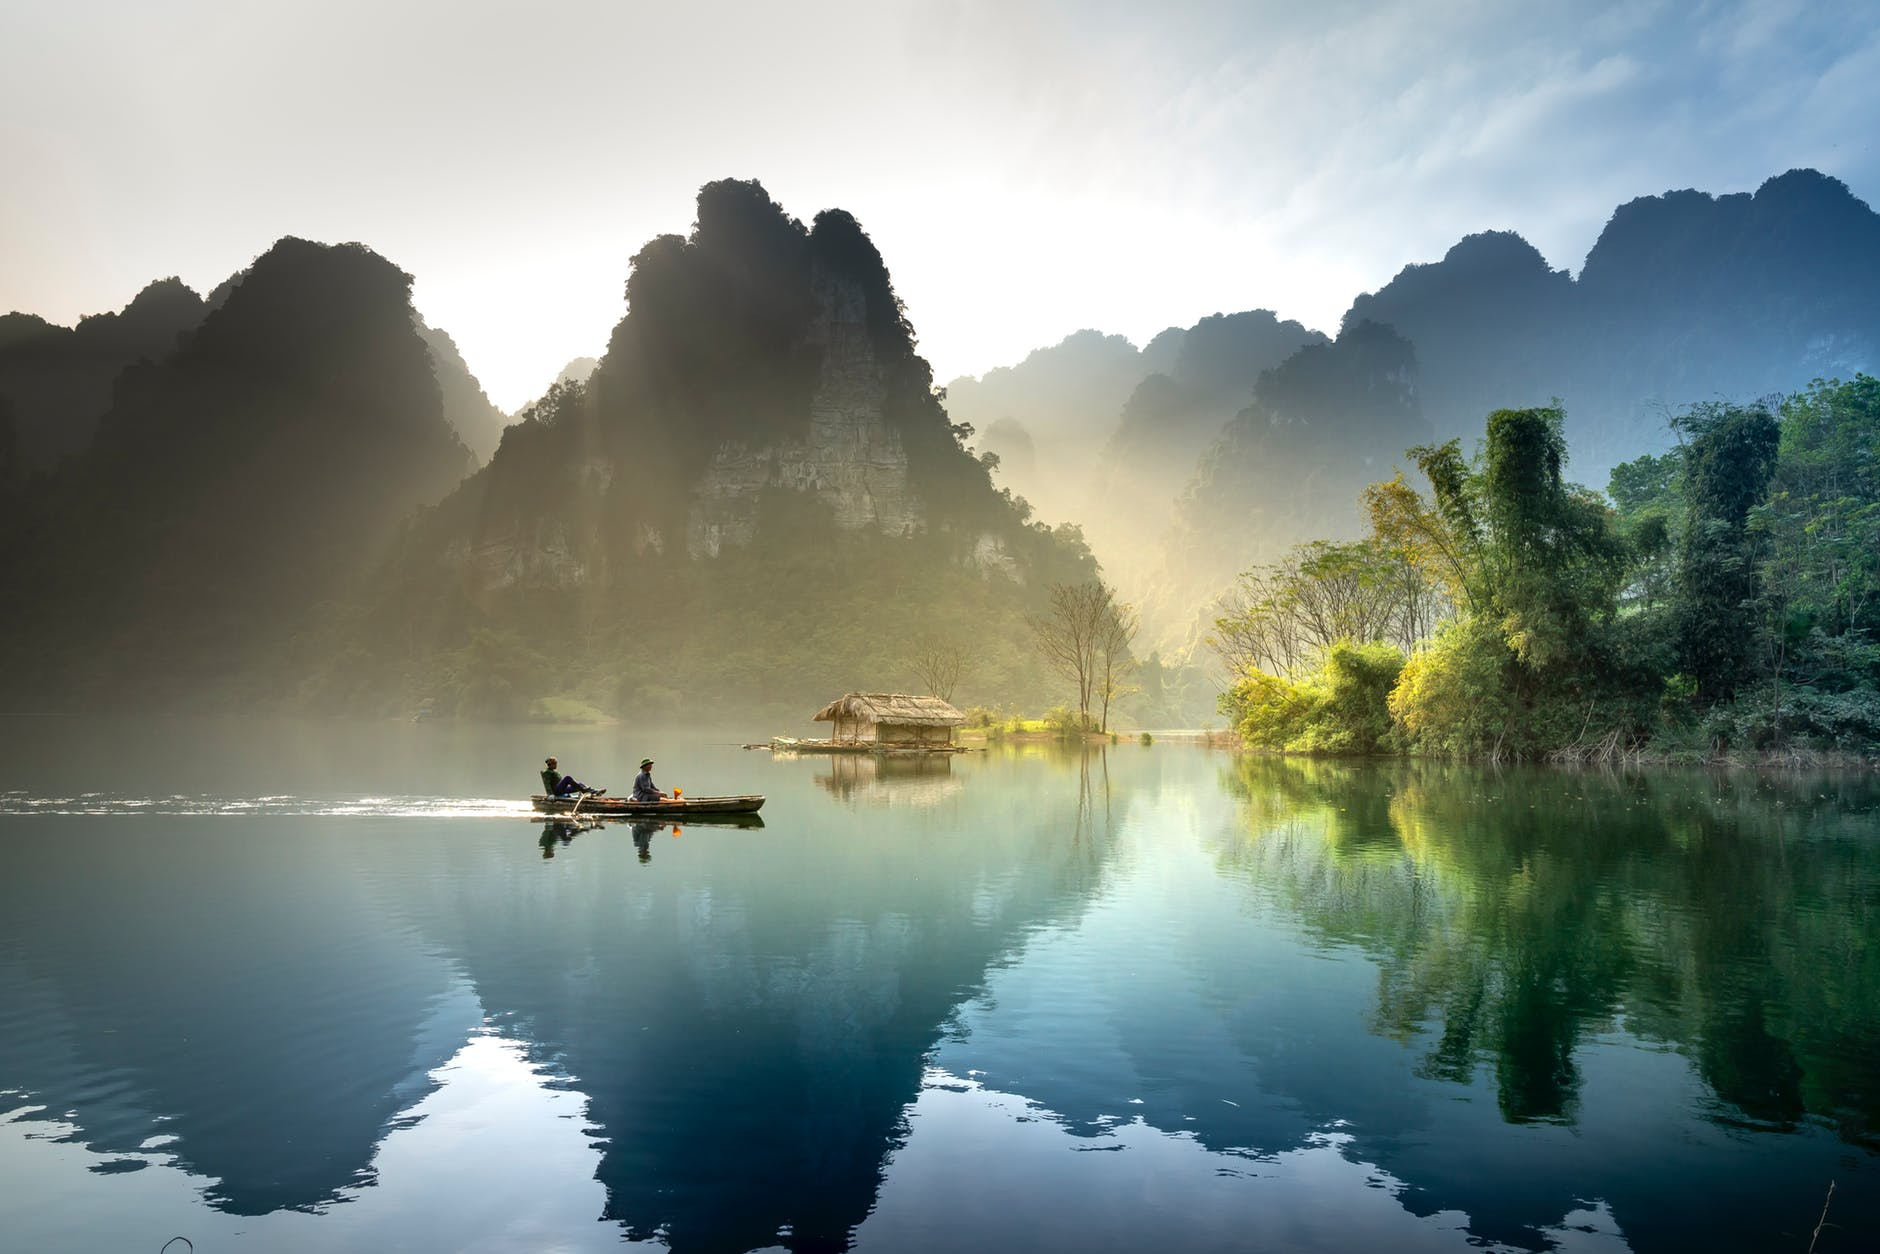
\includegraphics[width=0.5\textwidth]{lake.jpeg}
    \caption{多图片2}
    \label{fig:MultiPic2}
\end{figure}

\chapter{测试\the\baselineskip}
\the\baselineskip
\section{文字测试\the\baselineskip}

这是武汉大学学位论文模版,欢迎使用。\the\baselineskip

This is Wuhan University thesis template, welcome to use!\the\baselineskip

\section{公式\the\baselineskip}

\subsection{算符、希腊字母\the\baselineskip}

\[\sum\prod\int\iint\alpha\beta\gamma\xi\zeta\eta\epsilon\varepsilon\theta\vartheta
    \phi\varphi\psi \the\baselineskip\]

\subsection{几类数学字母表\the\baselineskip}

\begin{itemize}
    \item \verb|\mathcal|: $\mathcal{ABCDEFGHIJKLMNOPQRSTUVWXYZ}$ \the\baselineskip
    \item \verb|\mathscr|: $\mathscr{ABCDEFGHIJKLMNOPQRSTUVWXYZ}$ \the\baselineskip
    \item \verb|\mathbb|: $\mathbb{ABCDEFGHIJKLMNOPQRSTUVWXYZ}$ \the\baselineskip
\end{itemize}

\subsection{(不)带编号单行公式 \the\baselineskip}

Use \texttt{equation} environment: \the\baselineskip
\begin{equation}
    a^2 + b^2 = c^2. \the\baselineskip
\end{equation}
\the\baselineskip

Use \texttt{equation*} environment or \texttt{\textbackslash[...\textbackslash]}: \the\baselineskip
\[ a^2 + b^2 = c^2. \the\baselineskip\]
\the\baselineskip
\subsection{(不)带编号多行公式}

Use \texttt{align} environment:
\begin{align}
    S_n & = 1 + 2 + \cdots + n \\
        & = \frac12 n(n+1).
\end{align}

Use \texttt{align*} environment:
\begin{align*}
    T_n & = 1^3 + 2^3 + \cdots + n^3         \\
        & = \biggl(\frac{n(n+1)}{2}\biggr)^2 \\
        & = S_n^2.
\end{align*}

\subsection{矩阵}

\[
    \begin{pmatrix}
        a_{11} & a_{22} & a_{33} \\
        a_{21} & a_{22} & a_{23} \\
        a_{31} & a_{32} & a_{33} \\
    \end{pmatrix} \quad
    \begin{vmatrix}
        a_{11} & a_{22} & a_{33} \\
        a_{21} & a_{22} & a_{23} \\
        a_{31} & a_{32} & a_{33} \\
    \end{vmatrix} \quad
    \begin{bmatrix}
        a_{11} & a_{22} & a_{33} \\
        a_{21} & a_{22} & a_{23} \\
        a_{31} & a_{32} & a_{33} \\
    \end{bmatrix} \quad
    \begin{Bmatrix}
        a_{11} & a_{22} & a_{33} \\
        a_{21} & a_{22} & a_{23} \\
        a_{31} & a_{32} & a_{33} \\
    \end{Bmatrix}\]

\section{脚注测试}

测试 \footnote{眼看他起朱楼,眼看他宴宾客,眼看他楼塌了。这青苔碧瓦堆,俺曾睡风流觉,将五十年兴亡看饱。
    金粉未消亡,闻得六朝香,满天涯烟草断人肠。怕催花信紧,风风雨雨,误了春光。}

测试 \footnote[3]{君不见,左纳言,右纳史,朝承恩,暮赐死。行路难,不在水,不在山,只在人情反覆间!}

\section{引用测试}

\subsection{参考文献}

测试 \cite{huangzh,anon-cn1,anon-cn2,anon-cn3,anon-cn4,anon-cn5}

测试 \cite*{anon-en1,anon-en2,anon-en3,anon-en4,anon-en5}

注意手写参考文献和使用 bib 文件的样式有顶格不顶格的区别,由于没有详细要求,选一使用即可。

\section{图表测试}

\begin{figure}[ht]
    \centering
    
\includegraphics[width = 5cm]{gdufelogo.png}
    \caption{广东财经大学校徽}
    \label{fig:广东财经大学校徽}
\end{figure}

引用图~\ref{fig:广东财经大学校徽}

\begin{table}[ht]
    \centering
    \caption{%
        简单的表格和引用 abc 123 %\cite{whu-bachelor:1}
    }
    \label{table:简单的表格}
    \begin{tabular}{cc}
        \hline
        a  & b  \\ \hline
        c  & d  \\ \hline
        测试 & 文本 \\ \hline
    \end{tabular}
\end{table}

\begin{table}[ht]
    \centering
    \caption{%
        三线表格和引用 abc 123 %\cite{whu-bachelor:1}
    }
    \label{table:三线表格}
    \begin{tabular}{cc}
        \toprule
        列名1 & 列名2 \\ \midrule
        a   & b   \\
        c   & d   \\
        测试  & 文本  \\ \bottomrule
    \end{tabular}
\end{table}

引用表~\ref{table:简单的表格}
引用表~\ref{table:三线表格}

\section{算法}

\begin{algorithm}
    \caption{An algorithm with caption}\label{alg:cap}
    \begin{algorithmic}
        \Require $n \geq 0$
        \Ensure $y = x^n$
        \State $y \gets 1$
        \State $X \gets x$
        \State $N \gets n$
        \While{$N \neq 0$}
        \If{$N$ is even}
        \State $X \gets X \times X$
        \State $N \gets \frac{N}{2}$  \Comment{This is a comment}
        \ElsIf{$N$ is odd}
        \State $y \gets y \times X$
        \State $N \gets N - 1$
        \EndIf
        \EndWhile
    \end{algorithmic}
\end{algorithm}

引用 \autoref{alg:cap}

\section{已定义好的一些数学定理环境}

\begin{defi}[测度]
    (参见文献xxx) 这是一段文字 $E = m c^2$  (中文括号)和 (西文括号)
\end{defi}

\begin{theo}
    这是一段文字 $E = m c^2$
\end{theo}

\begin{proof}
    这是一段文字 $E = m c^2$
\end{proof}

\begin{proof}[定理xx的证明]
    这是一段文字 $E = m c^2$
\end{proof}

\begin{exam}
    这是一段文字 $E = m c^2$
\end{exam}

\begin{prop}
    这是一段文字 $E = m c^2$
\end{prop}

\begin{coro}
    这是一段文字 $E = m c^2$
\end{coro}

\begin{lemm}
    这是一段文字 $E = m c^2$
\end{lemm}

\begin{rema}
    这是一段文字 $E = m c^2$
\end{rema}

\begin{theo}[Banach-Steinhaus]\label{thm:test}
    设 $E$ 是 Banach 空间, $F$ 是赋范空间, $(u_i)_{i\in I}$ 是一族从 $E$ 到 $F$ 的有界线性算子,
    即 $(u_i)_{i\in I}\subset \mathcal{B}(E,F)$. 若对每一点 $x\in E$, 有
    $\sup_{i\in I} \|u_i(x)\|<\infty$, 则
    \begin{equation}\label{eq:test1}
        \sup_{i\in I} \|u_i\| < \infty.
    \end{equation}
\end{theo}

我想引用定理~\ref{thm:test} 和公式~\ref{eq:test1}

定理括号测试:

\begin{theo}
    测试
    \begin{enumerate}
        \item 中文(括号)没输入空格的效果
        \item 中文 (括号) 输入空格的效果
        \item 西文(括号)没输入空格的效果
        \item 西文 (括号) 输入空格的效果
    \end{enumerate}
\end{theo}

\begin{proof}
    test
    \[
        \int_{0}^{1} x^2 \d x
    \]
\end{proof}

% \begin{proof}
%   test
%   \[
%     \int_{0}^{1} x^2 \d x \qedhere
%   \]
% \end{proof}

\section{字体测试}
字体测试:

\begin{table}[ht]\centering
    \begin{tabular}{lll}
        \toprule
        命令               & 宋体效果                & Times New Roman 效果                       \\
        \midrule
        \verb|\rmfamily| & {\rmfamily 宋体罗马字族}  & {\rmfamily Times New Roman Roman Family} \\
        \verb|\sffamily| & {\sffamily 宋体无衬线字族} & {\sffamily Times New Roman Sans Serif}   \\
        \verb|\ttfamily| & {\ttfamily 宋体打字机}   & {\ttfamily Times New Roman Typewriter}   \\
        \verb|\bfseries| & {\bfseries 宋体加粗}    & {\bfseries Times New Roman Bold}         \\
        \verb|\itshape|  & {\itshape 宋体意大利}    & {\itshape Times New Roman Italic}        \\
        \verb|\slshape|  & {\slshape 宋体倾斜}     & {\slshape Times New Roman Slanted}       \\
        \bottomrule
    \end{tabular}
    \caption{宋体与 Times New Roman 字体命令效果对比}
\end{table}

\begin{table}[ht]
    \centering
    \begin{tabular}{cccccc}
        \toprule
        测试类型 & {\songti 宋体}             & {\heiti 黑体}                    & {\kaishu 楷书}                    & {\fangsong 仿宋}                    & Times new roman               \\
        \midrule
        伪粗体  & {\bfseries 字体测试}         & {\bfseries\heiti 字体测试}         & {\bfseries\kaishu 字体测试}         & {\bfseries\fangsong 字体测试}         & {\bfseries Font test}         \\
        伪斜体  & {\itshape 字体测试}          & {\itshape\heiti 字体测试}          & {\itshape\kaishu 字体测试}          & {\itshape\fangsong 字体测试}          & {\itshape Font test}          \\
        叠加测试 & {\bfseries\itshape 字体测试} & {\bfseries\itshape\heiti 字体测试} & {\bfseries\itshape\kaishu 字体测试} & {\bfseries\itshape\fangsong 字体测试} & {\bfseries\itshape Font test} \\
        \bottomrule
    \end{tabular}
    \caption{不同字体下伪粗体、伪斜体及叠加效果测试}
\end{table}

Lorem ipsum dolor sit amet, consectetur adipiscing elit, sed do eiusmod tempor incididunt ut labore et dolore magna aliqua. Ut enim ad minim veniam, quis nostrud exercitation ullamco laboris nisi ut aliquip ex ea commodo consequat. Duis aute irure dolor in reprehenderit in voluptate velit esse cillum dolore eu fugiat nulla pariatur.Lorem ipsum dolor sit amet, consectetur adipiscing elit, sed do eiusmod tempor incididunt ut labore et dolore magna aliqua. Ut enim ad minim veniam, quis nostrud exercitation ullamco laboris nisi ut aliquip ex ea commodo consequat. Duis aute irure dolor in reprehenderit in voluptate velit esse cillum dolore eu fugiat nulla pariatur.


%%%============正文之后的页眉页脚格式========%%%
\cleardoublepage
\phantomsection
\appendix
%%%=== 参考文献 ========%%%
% % 手写参考文献
\begin{thebibliography}{00}
    \bibitem {huangzh}黄正华. \url{http://aff.whu.edu.cn/huangzh/}.
    \bibitem{r1} 作者. 文章题目 [J].  期刊名, 出版年份,卷号(期数): 起止页码.
    \bibitem{r2} 作者. 书名 [M]. 版次. 出版地:出版单位,出版年份:起止页码.
    \bibitem{r3} 邓建松等, 《\LaTeXe~科技排版指南》, 科学出版社.
    \bibitem{r4} 吴凌云, 《CTeX~FAQ (常见问题集)》, \textit{Version~0.4}, June 21, 2004.
    \bibitem{r5} Herbert Vo\ss, Mathmode, \url{http://www.tex.ac.uk/ctan/info/math/voss/mathmode/Mathmode.pdf}.
    \bibitem{anon-cn1} 匿名. 关于人工智能发展的若干思考[J]. 计算机科学, 2022, 49(6): 1-10.
    \bibitem{anon-cn2} 匿名. 区块链技术及其应用前景分析[J]. 信息技术, 2023, 47(2): 45-47.
    \bibitem{anon-cn3} 匿名. 现代城市交通管理系统研究[M]. 北京: 科学出版社, 2021.
    \bibitem{anon-cn4} 匿名. 论大数据时代的隐私保护问题[C]// 全国网络安全学术会议论文集. 2020: 123-134.
    \bibitem{anon-cn5} 匿名. 机器学习在医学影像分析中的应用综述[J]. 医学信息, 2024, 37(5): 88-92.
    \bibitem{anon-en1} Anonymous. A brief review of deep learning techniques[J]. Journal of Artificial Intelligence, 2023, 15(4): 201-210.
    \bibitem{anon-en2} Anonymous. Blockchain: Opportunities and Challenges[C]// Proceedings of the International Conference on Computer Science. 2022: 55-60.
    \bibitem{anon-en3} Anonymous. Smart City: Concepts and Realizations[M]. New York: Tech Press, 2020.
    \bibitem{anon-en4} Anonymous. Privacy Issues in the Age of Big Data[J]. Information Security, 2021, 12(3): 77-80.
    \bibitem{anon-en5} Anonymous. Machine Learning Applications in Medical Imaging: A Survey[J]. Medical Informatics, 2024, 18(2): 99-105.
\end{thebibliography}
%% 添加参考文献到电子书签
\addcontentsline{toc}{chapter}{参考文献}

%% 使用bib 文件管理参考文献,不使用请删除
\printbibliography[heading=bibintoc, title={参考文献--bib}]

\chapter{攻读硕士学位期间取得的研究成果}
\begin{list}{[\arabic{enumi}]}{\usecounter{enumi}}
    \item Author3, "Title3", Journal3, Volume3, Pages3, Year3.
    \item Author4, "Title4", Conference4, Location4, Year4.
          % 其他成果条目
\end{list}

\chapter{附录测试2}

\section{测试2.1}

测试
\section{测试2.2}

测试

\cleardoublepage
% !Mode:: "TeX:UTF-8"
%%%%%%%%%%%%%%%%%%%%%%%%%%%%-------致谢--------%%%%%%%%%%%%%%%%%%%%%%%%%%%%%%%%
% 致谢居中
\chapter*{{ }\hfill\ziju{2}{致谢}\hfill{ }}
\addcontentsline{toc}{chapter}{致谢}

饮水思源. 衷心感谢武汉大学黄正华教授提供的武汉大学本科毕业论文的源代码. 本模板是在上述代码的基础上结合广东财经大学毕业论文格式规范进行修改得到的.

祝愿大家:Happy texing!
 %%%致谢
\end{document}